\documentclass[a4paper,11pt,twoside]{article}
%\documentclass{report}
% Per encoding dei caratteri: così com'è permette lettere accentate in input
\usepackage[T1]{fontenc}
\usepackage[utf8]{inputenc}
%\usepackage[latin1]{inputenc}

\usepackage{multicol, caption}
\usepackage{booktabs}
\usepackage{gensymb}
\usepackage[usenames,dvipsnames]{xcolor}
\usepackage{xfrac}
\usepackage{footnote}
\usepackage{textcomp}
\usepackage{dsfont}
\usepackage[italian]{babel}
\usepackage{graphicx}
\usepackage{tabularx}
\usepackage{vmargin}
%\usepackage{multicol}
% \usepackage{subfigure}
\usepackage{caption}
% \usepackage{subcaption}
% \usepackage{upgreek}
\usepackage{rotating}
\usepackage{amssymb}
\usepackage{amsmath}
\usepackage{amsthm}
\usepackage{mathtools}
\usepackage{lscape}
%\usepackage{subfig}
\usepackage{subfigure}
\usepackage{pgfplots}
\usepackage{tikz}

% Comodità da eliminare alla stampa
%\usepackage{showkeys}
%\usepackage[pdftex]{hyperref} 

% Comandi utili ( ridefiniti: \u,\v,\O )
\newcommand{\vertiii}[1]{{\left\vert\kern-0.25ex\left\vert\kern-0.25ex\left\vert #1 
    \right\vert\kern-0.25ex\right\vert\kern-0.25ex\right\vert}}
\newcommand{\Q}{Q^{ad}}
\renewcommand{\u}{\mathbf{u}}
\renewcommand{\v}{\mathbf{v}}
\newcommand{\z}{\mathbf{z}}
\newcommand{\du}{\mathbf{\delta u}}
\newcommand{\tu}{\mathbf{\tau u}}
\newcommand{\dq}{{\delta q}}
%\newcommand{\dp}{\delta p}	% ridefinirlo dà problemi
\newcommand{\qs}{{q_\sigma}}
\newcommand{\weak}{\rightharpoonup}
\renewcommand{\O}{{\Omega_0}}
\newcommand{\Oq}{{\Omega_q}}
\newcommand{\beq}{\begin{equation}}
\newcommand{\eeq}{\end{equation}}

% Teoremi & co.
\theoremstyle{plain}
\newtheorem{teor}{Teorema}[section]
\newtheorem{cor}[teor]{Corollario}
\newtheorem{lemma}[teor]{Lemma}
\newtheorem{prop}[teor]{Proposizione}

\theoremstyle{definition}
\newtheorem{assunzione}[teor]{Ipotesi}

\theoremstyle{remark}
\newtheorem{oss}{Osservazione}

%\graphicspath{{C:\Users\Ivan\Documents\Polimi\AA 2012-13\I Semestre\PACS\Condivisa_con_xubuntu-pacs\per_Fis_Tec}}
%\graphicspath{C:\Users\Ivan\Dropbox\FisicaTecnica_gruppo6\Elaborato3}
%\DeclareGraphicsExtensions{.pdf,.ps,.eps,.png,.jpeg,.mps}
%
%\bibliographystyle{plain}
%\bibliography{C:/Users/Ivan/Documents/library}

%\setmarginsrb{10mm}{5mm}{10mm}{10mm}%
%             {0mm}{10mm}{0mm}{10mm}

%%%%%%%
%G%		è il commento nel caso di Stokes generalizzato (avevo sbagliato: avevo messo il dato di Dirichlet in rhs anche all'eq della div)

\begin{document}


%%%%%%%%%%%%%%%%%%%%%%%%%%%%%%%%%%%%%%%%%%%%%%%%%%%%%%%%%%%%
%%%%%%%%%%%%%%%%%%%%%%%%%%%%%%%%%%%%%%%%%%%%%%%%%%%%%%%%%%%%
\section{Analisi di un problema di controllo per flusso di Stokes}

\begin{oss}
	Quando nelle stime che seguono comparirà una costante $c$, la si intenderà dipendente solo dai dati, e non dal controllo $q$, dalle variabili di stato $\u,p$, né da loro variazioni e nemmeno dai parametri di discretizzazione $\sigma,h$. Ciò varrà anche dove vi sia un utilizzo della disuguaglianza di Poincaré, dal momento che le costanti relative a ciascun $\Omega_q$ sono tutte controllate da quella relativa a quel dominio $\hat{\Omega}$ che li contiene tutti.
\end{oss}
%SISTEMARE TUTTO CIO' CHE PARLA DEL RILEVAMENTO E VEDERE SE C'E' RILEVAMENTO ANCHE NELL'EQ DI CONTINUITA'
%%%%%%%%%%%%%%%%%%%%%%%%%%%%%%%%%%%%%%%%%%%%%%%%%%%%%%%%%%%%
\subsection{Definizione del problema}\label{sec:def}

%%%%%%%%%%%%%%%%%%%%%%
%%\begin{figure}[htbp,width=0.9\textwidth]
%\begin{center}
%	\begin{tikzpicture}
%	\begin{axis}
%		[xmin=0,xmax=1,ymin=0,ymax=1,xtick={0,1},ytick={0,1},
%		xlabel=$x$,ylabel=$y$,title={Dominio fisico $\Oq$},
%		width=0.3\textwidth]
%	\end{axis}
%	\end{tikzpicture}
%	\hfill
%	\begin{tikzpicture}
%	\begin{axis}
%		[xmin=0,xmax=1,ymin=0,ymax=1,xtick={0,1},ytick={0,1},
%		xlabel=$x$,ylabel=$y$,title={Dominio di riferimento $\O$},
%		width=0.3\textwidth]
%	\end{axis}
%	\end{tikzpicture}
%\end{center}
%%\end{figure}
%%\\

%\begin{figure}
%	\begin{subfigure}
%		\includegraphics[draft=true]{Omegaq.jpg}
%		\caption{Dominio fisico $\Oq$}
%		\label{fig:Oq}
%	\end{subfigure}
%	\begin{subfigure}
%		\includegraphics[draft=true]{Omega0.jpg}
%		\caption{Dominio fisico $\O$}
%		\label{fig:O0}
%	\end{subfigure}
%\end{subfloat}

\begin{figure}[h]
	\centering
	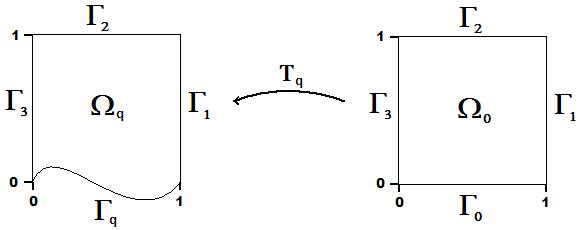
\includegraphics[width=0.7\textwidth]{img/Domini.jpg}
	\caption{Dominio fisico e dominio di riferimento}
\label{fig:domini}
\end{figure}
%%%%%%%%%%%%%%%%%%%%%%
Siano $q:I=(0,1)\to\mathds{R}$, $\Omega_q =\{(x,y)\in \mathds{R}^2\ |\ x\in I\ ,\ y\in (q(x),1)\}$ e partizioniamo il bordo di $\Omega_q$ come indicato in Figura \ref{fig:domini}: $\partial\Omega_q=\Gamma_q\cup\Gamma_1\cup\Gamma_2\cup\Gamma_3$.\\
Per evitare domini degeneri, fissiamo a priori $\varepsilon\in(0,1)$ e definiamo come insieme dei controlli $\overline{Q}^{ad}=\{q\in H^2(I)\cap H^1_0(I)\ |\ q(x)\leq 1-\varepsilon \ \forall x\in I \}$.\\
Consideriamo il problema di Stokes in $\mathbf{u}=(u,v)$ e $p$
\begin{equation}
\left\{
\begin{aligned}
	\eta \mathbf{u} - div(\nu\nabla\mathbf{u}) + \nabla p &= \mathbf{f} \qquad &in\ \Omega_q\\
	div\ \mathbf{u} &= 0 \qquad &in\ \Omega_q\\
	\mathbf{u} &= 0 \qquad &su\ \Gamma_q\\
	\nu\partial_\mathbf{n }\mathbf{u} - p \mathbf{n} &= \mathbf{g}_N\qquad &su\ \Gamma_1\\%=\partial\Omega_q\backslash\Gamma_D
	\partial_\mathbf{n} u = 0,\quad v&=0\qquad &su\ \Gamma_2\\
	\mathbf{u} &= \mathbf{g}_D\qquad &su\ \Gamma_3\\% \subset\partial\Omega_q\\
\end{aligned}
\right.
\label{eq:Stokes}
\end{equation}
dove i dati $\eta,\nu,\mathbf{f}$ siano definiti su $\hat{\Omega}: \Omega_q\subseteq\hat{\Omega}\quad\forall q\in \overline{Q}^{ad}$.\\
Definendo $\widetilde{\mathcal{R}}\mathbf{g}_D$ come un rilevamento continuo di $\mathbf{g}_D$ su $\Omega_q$ e gli spazi
\begin{equation*}\begin{split}
	\widetilde{V}&=\{\v\in[H^1(\Oq)]^2\colon \v=(v_x,v_y)=\mathbf 0\text{ su }\Gamma_3\cup\Gamma_q\text{ e }v_y=0\text{ su }\Gamma_2\}\\
	\widetilde{P}&=L^2(\Oq)
\end{split}\end{equation*}
la formulazione debole del problema \`e
\begin{equation}
\begin{split}
	\text{Trovare }\mathbf{u} = \mathbf{\hat{u}}+\widetilde{\mathcal{R}}\mathbf{g}_D \ ,\ \mathbf{\hat{u}}\in V=[H^1_{\Gamma_3}(\Omega_q)]^2 \text{ e } p\in P=L^2(\Omega_q)\text{ tali che } \\
	\left\{
	\begin{aligned}
		a_q(\mathbf{\hat{u}},\mathbf{v}) + b_q(\mathbf{v},p) &= F_q(\mathbf{v})\qquad&\forall\ \mathbf{v}\in  [H^1_{\Gamma_3}(\Omega_q)]^2\\
		b_q(\mathbf{\hat{u}},\pi) &= -b_q(\widetilde{\mathcal{R}}\mathbf g_D,\pi)
				\qquad&\forall\ \pi \in L^2(\Omega_q)\\
	\end{aligned}\right.\\
	\begin{split}
	\text{dove } a_q(\mathbf{u},\mathbf{v}) &=\int_{\Omega_q}{\eta \mathbf{u}\mathbf{v}+\nu\nabla \mathbf{u}:\nabla\mathbf{v}}\\
		b_q(\mathbf{v},\pi) &= -\int_{\Omega_q}{\pi\ div\ \mathbf{v}}\\
		F_q(\mathbf{v}) &= \int_{\Omega_q}{ \mathbf{f}\cdot \mathbf{v}}-a_q(\widetilde{\mathcal{R}}\mathbf{g}_D,\mathbf{v}) + \int_{\Gamma_1}{\mathbf{g}_N\cdot\mathbf{v}\,d\Gamma}\\
		%G%G_q(\pi)=-b_q(\mathcal{R}\mathbf{g}_D,\pi)\\
	\end{split}
\end{split}
\label{eq:Stokesdeb}
\end{equation}
Affinch\'e questo problema sia ben posto sono necessarie alcune condizioni sui dati, che qui riportiamo:\footnote{A $q$ fissato, basterebbe che le condizioni fossero verificate relativamente ad $\Omega_q$, ma per non dover dipendere dal controllo, consideriamo $\hat{\Omega}$.}
\begin{itemize}
	\item $\nu(x,y)\geq\nu_0>0\ \ \forall (x,y)\in\hat{\Omega}$ \ per assicurare la coercivit\`a di $a_q$
	\item $\nu,\eta\in L^\infty(\hat{\Omega})$ per avere la continuit\`a di $a_q$ (quella di $b_q$ non necessita di richieste sui dati)
	\item $\mathbf{f}^q\in H^{-1}(\hat{\Omega}),\ \mathbf g_D\in H^{1/2}(\Gamma_3),\ \mathbf g_N\in L^2(\Gamma_1)$ per la continuità del funzionale a termine noto
\end{itemize}
Queste condizioni garantiscono anche, attraverso le classiche stime di stabilità, che\\$\|(\u,p)\|_{[H^1_0(\Oq)]^2\times L^2(\Oq)}$ sia limitata da una costante dipendente dai dati, uniformemente rispetto a $q$. Inoltre permettono che sia ben definito l'operatore soluzione $\widetilde{S}(q)$, che associa ad ogni $q\in\overline{Q}^{ad}$ la corrispondente soluzione $(\mathbf{u},p)=\widetilde{S}(q)$ del problema di stato.

Definito il problema di stato \eqref{eq:Stokes}, fissiamo due costanti $\alpha,\beta>0$ per penalizzare rispettivamente la derivata seconda di $q$ e il vincolo di volume costante sotteso a $q$. Il problema di ottimizzazione di forma che vogliamo affrontare \`e il seguente:
\begin{equation}
	\begin{aligned}
	\text{Minimizzare } J(q,\mathbf{u},p) = \frac{1}{2}\int_{\Omega_q}{|\nabla \mathbf{u}|^2} + \frac{\alpha}{2}\|q''\|_{L^2(I)}^2 +	\frac{\beta}{2}\left(\int_I {q(x)dx} - \overline{V}\right)^2\\
	\text{soggetto al vincolo \eqref{eq:Stokes}}
	\end{aligned}
\label{eq:minJ}
\end{equation}
Utilizzando l'operatore soluzione appena introdotto, possiamo considerare anche il funzionale di costo ridotto $j:\overline{Q}^{ad}\rightarrow\mathds{R}:q\mapsto j(q)=J(q,\widetilde{S}(q))$.

Considerando $q_0\equiv 0 \in \overline{Q}^{ad}$, possiamo affermare che una condizione necessaria affinch\'e una $q\in\overline{Q}^{ad}$ sia soluzione ottima del problema \`e che sia $j(q)\leq j(q_0)$, il che implica
$$ \|q''\|_{L^2(I)}^2 \leq \frac{2}{\alpha}\left[j(q_0)-  \frac{1}{2}\int_{\Omega_q}{|\nabla \mathbf{u}|^2} - \frac{\alpha}{2}\|q''\|_{L^2(I)} - \frac{\beta}{2}\left(\int_I {q(x)dx} - \overline{V}\right)^2\right] \leq \frac{2}{\alpha}j(q_0)$$
Poich\'e in $H^2(I)\cap H^1_0(I)$ la seminorma $H^2(I)$ \`e equivalente alla norma completa (Lemma 1.2 \cite{Kinigera}), ne risulta che possiamo considerare come insieme dei controlli ammissibili anche solo il sottoinsieme di $\overline{Q}^{ad}$ definito come
$$ Q^{ad} = \{q\in \overline{Q}^{ad}\ |\ \|q\|_{H^2(I)}\leq C=\frac{2}{\alpha}j(q_0)\} $$
Per gli studi di regolarit\`a, richiediamo anche che
\beq
	\exists d_1,d_2>0 \text{ tali che } \|q''\|_{L^\infty(I)}\leq d_1,\ |q'(0)|\leq d_2
\label{eq:Bad}
\eeq
%mentre per seguire le indicazioni di \cite{Kinigera} assumiamo anche che
%$$ \exists \varepsilon\in(0,1)\text{ tale che } q(x)\leq 1-\varepsilon \quad \forall x\in I $$


%%%%%%%%%%%%%%%%%%%%%%%%%%%%%%%%%%%%%%%%%%%%%%%%%%%%%%%%%%%%
\subsection{Esistenza}\label{sec:esistenza}

Per mostrare l'esistenza di una soluzione del problema \eqref{eq:minJ}, cominciamo con l'osservare che
$$J(q,\mathbf{u},p)\geq 0,\ Q^{ad}\neq\emptyset\quad\Rightarrow\quad \exists \{q_n\}_{n\in\mathds{N}} :\ \overline{j}:=\inf_{q\in Q^{ad}}j(q) = \lim_{n\in\mathds{N}}j(q_n)$$
La limitatezza di $\Q$ garantisce che, a meno di sottosuccessioni, $q_n\weak \overline{q}$ in $H^2(I)$; inoltre, dal momento che $\Q$ è anche convesso e chiuso, $\overline{q}\in\Q$.\\
% PARTE NON NECESSARIA SE J E' DEB.S.C.I.
%%%per ragioni notazionali, introduciamo l'operatore complessivo
%%% $$ \mathcal{A}_q:  [[H^1_0(\Omega_q)]^2\times L^2(\Omega_q)]^2 \rightarrow \mathds{R}:(\mathbf{u},p,\mathbf{v},\pi) \mapsto
%%%	\begin{pmatrix}
%%%		a_q(\mathbf{u},\mathbf{v}) + b_q(\mathbf{v},p)\\
%%%		b_q(\mathbf{u},\pi)
%%%	\end{pmatrix}
%%%$$
%%%e verifichiamo la validit\`a delle seguenti propriet\`a:		
%%%\begin{itemize}
%%%	\item[A1] Uniforme continuit\`a di $\mathcal{A}_q(\mathbf{u},p,\mathbf{v},\pi)\ \forall q\in Q$\\
%%%		Basta richiedere che siano $\eta,\nu\in L^\infty(\hat\Omega)$
%%%	\item[A2] Uniforme coercivit\`a di $\mathcal{A}_q(\mathbf{u},p,\mathbf{v},\pi)\ \forall q\in Q$\\
%%%		Basta richiedere che sia $\nu\geq\nu_0>0$.
%%%		\textcolor{red}{CONSIDERIAMO $\Gamma_n=\emptyset$}
%%%	\item[A3] Simmetria di $\mathcal{A}_q(\mathbf{u},p,\mathbf{v},\pi)\ \forall q\in Q$\\Non \`e verificata, ma non \`e necessaria (cfr. \emph{Remark 2.9}).
%%%	\item[A4] Continuit\`a di $q\mapsto \mathcal{A}_q$ (cfr. \emph{Remark 2.9})\\
%%%		Conseguenza della uniforme continuit\`a, della dipendenza continua dell'integrale dal dominio e della limitatezza di $\|q\|_{H^2(I)}$: si verifica la continuit\`a rispetto a $q$ di $a_q$ e $b_q$ separatamente come nel caso ellittico, e quella di $A_q$ \`e implicata.
%%%\end{itemize}
%%%Sotto queste ipotesi, possiamo formulare per il nostro problema un analogo del Lemma 2.12 [Haslinger]
%%%\begin{lemma}
%%%	Siano $\{q_n\}\in Q^{ad}: q_n\to_{L^\infty(I)} q\in Q^{ad}$ e $(\mathbf{u}_n,p_n)=\widetilde{S}(q_n)\in [H^1_0(\Omega_q)]^2\times L^2(\Omega_q)$.
%%%	Sotto le ipotesi (A1)--(A4) si ha che $\exists (\mathbf{\hat{u}},\hat{p}) \in [H^1_0(\Omega_q)]^2\times L^2(\Omega_q): (\mathbf{u}_n,p_n)\to (\mathbf{\hat{u}},\hat{p})\text{ in }[H^1_0(\Omega_q)]^2\times L^2(\Omega_q)$ e $(\mathbf{\hat{u}},\hat{p})
%%%\end{lemma}
La dimostrazione del Teorema 2.1 \cite{Gunzburger2000}, poi, a partire dall'uniforme limitatezza di $\widetilde{S}(q_n)$ in $[H^1(\hat{\Omega})]^2\times L^2(\hat{\Omega})$, ci assicura che $\widetilde{S}(q_n)$ converga debolmente ad una coppia $(\overline{\u},\overline{p})$ che sia proprio $\widetilde{S}(\overline{q})$.\\
Per poter passare al limite nel funzionale, poich\'e la successione \`e minimizzante, \`e sufficiente che $J(q,\mathbf{u},p)$ sia debolmente semicontinuo inferiormente su $H^2(I)\times [H^1_0(\Omega_q)]^2\times L^2(\Omega_q)$: ci\`o \`e garantito dalla debole semicontinuit\`a inferiore delle norme, dal Teorema 1.2 \cite{Gunzburger2000} e dal Teorema della Convergenza Dominata (quest'ultimo per passare al limite nel termine di penalizzazione del volume).%@%\textcolor{red}{FORSE CONVIENE AMPLIARE UN PO' QUESTA PARTE.}


%%%%%%%%%%%%%%%%%%%%%%%%%%%%%%%%%%%%%%%%%%%%%%%%%%%%%%%%%%%%
\subsection{Trasformazione da $\Omega_q$ a $\Omega_0$}\label{sec:trasformazione}

Consideriamo come dominio di rifermento $\Omega_0=(0,1)^2$, che corrisponde a prendere $q\equiv 0$: \`e cos\`i possibile definire una mappa
$$T_q :\Omega_0\rightarrow\Omega_q:(x,y)\mapsto \begin{pmatrix}x\\y+(1-y)q(x)\end{pmatrix}$$
Per le espressioni delle altre grandezze legate a questa mappa ($V_q=T_q-\mathds{1},DT_q,\gamma_q=det(DT_q),A_q=\gamma_qDT_q^{-1}DT_q^{-T}$) si vedano le definizioni a pagina 6 di \cite{Kinigera}.\\
\begin{itemize}
\item[\underline{NB}]%Qualora non vi siano dubbi sulla $q$ scelta, indichiamo con $\widetilde{\cdot}$ le grandezze con dominio in $\Omega_q$, mentre non diamo alcuna notazione particolare a quelle con dominio in $\Omega_0$.
Indichiamo con apice $\cdot^q$ la composizione con la mappa $T_q$, mentre, qualora non vi siano dubbi sulla $q$ utilizzata, indichiamo con $\widetilde{\cdot}$ la composizione con $T_q^{-1}$; in altre parole, data una qualsiasi $\varphi:\Omega_q\rightarrow\mathds{R}$, definiamo $\varphi^q=\varphi \circ T_q:\Omega_0\to\mathds{R}\text{, mentre sarà ad esempio }\widetilde{\u}=\u\circ T_q^{-1}$ quando $\u$ sarà la soluzione del problema trasformato.\\
Inoltre, con $(\cdot,\cdot)$ intendiamo il prodotto scalare in $[L^2(\Omega_0)]^d$ (con $d$ che si pu\`o evincere dal contesto) e con $(\cdot,\cdot)_I$ e $(\cdot,\cdot)_\Oq$ rispettivamente quello in $L^2(I)$ e quello in $L^2(\Oq)$.
\end{itemize}
Possiamo dunque trasformare il nostro problema variazionale di partenza utilizzando spazi che non dipendono pi\`u da $q$, in quanto definiti su $\Omega_0$:\footnote{Nel caso \emph{fully Dirichlet} la dipendenza da $q$ rimane comunque, in quanto nella formulazione iniziale bisogna utilizzare $L^2_0(\Omega_q)$, che nella trasformata diventa $L^2_{\gamma_q^2}(\Omega_0)$, ossia il complemento ortogonale di $span\{\gamma_q^2\}$ in $L^2(\Omega_0)$.}\\
\begin{equation}
\begin{split}
	\text{Trovare }(\mathbf{u},p)\in V\times P, \text{ tale che } \\
	\left\{
	\begin{aligned}
		a(q)(\mathbf{u},\mathbf{v}) + b(q)(\mathbf{v},p) &= F(q)(\mathbf{v})\qquad&\forall\ \mathbf{v}\in  V\\
		b(q)(\mathbf{u},\pi) &= G(q)(\pi)
			\qquad&\forall\ \pi \in P\\
	\end{aligned}\right.\\
	\begin{split}
		\text{dove } a(q)(\mathbf{u},\mathbf{v})&=\int_{\Omega_0}{\eta^q \mathbf{u}\cdot\mathbf{v}\gamma_q+\nu^q\ tr(\nabla \mathbf{u}A_q\nabla\mathbf{v}^T)}\\
		b(q)(\mathbf{v},\pi) &= -\int_{\Omega_0}{\pi\ tr(\nabla\mathbf{v}DT_q^{-1})\gamma_q}\\
		F(q)(\mathbf{v}) &= \int_{\Omega_0}{ \mathbf{f}\cdot \mathbf{v}\ \gamma_q}-a(q)(\mathcal{R}\mathbf{g}_D,\mathbf{v}) + \int_{\Gamma_1}{\mathbf{g}_N\cdot\mathbf{v}\,d\Gamma}\\
		G(q)(\pi)&=-b(q)(\mathcal{R}\mathbf{g}_D,\mathbf{v})\\
		V&=\{\v\in[H^1(\O)]^2\colon \v=(v_x,v_y)=\mathbf 0\text{ su }\Gamma_3\cup\Gamma_0\text{ e }v_y=0\text{ su }\Gamma_2\}\\
		P&=L^2(\O)
	\end{split}\\
\end{split}
\label{eq:StokesdebT}
\end{equation}
Risulterà utile anche la definizione del seguente spazio (il corrispettivo discreto sarà analogo):
$$ V_{b(q)} = \{\v\in V\colon b(q)(\v,\pi) = 0\quad\forall q\in\Q\} $$
\begin{oss}[Rilevamento]
	Con $\mathcal{R}\mathbf g_D$ indichiamo un rilevamento continuo del dato di Dirichlet sul dominio $\O$. Notiamo che non è necessario trasformare $\mathbf g_D$ per riportarlo nel dominio di riferimento, dal momento che è definito sul bordo $\Gamma_3$, su cui la mappa $T_q$ è uguale all'identità. Ovviamente, a priori $\mathcal{R}\mathbf g_D\neq\widetilde{\mathcal{R}}\mathbf g_D\,\circ\,T_q$, ma ciò non importa, in quanto non utilizzeremo mai la forma del rilevamento.
\end{oss}
Per la buona positura del problema possiamo rifarci ancora alla teoria dei problemi di punto-sella ed affermare che sono sufficienti le richieste fatte per il problema non trasformato, dal momento che $A_q$ è in $[L^\infty(\O)]^{2\times2}$, simmetrica, definita positiva e il minimo autovalore è limitato inferiormente da $\overline{\lambda}=2\left(1+\frac{1+(d_1+d_2)^2}{\varepsilon} + \sqrt{\left(1+\frac{1+(d_1+d_2)^2}{\varepsilon}\right)^2-4}\right)^{-1}$
%E SUPPONIAMO CHE ABBIA AUTOVALORE MINIMO INFERIORMENTE LIMITATO DA UNA COSTANTE $\overline{\lambda}$ INDIPENDENTE DA q (TESTO IN ROSSO E' FALSO) \textcolor{red}{e con autovalori inferiormente limitati dalla costante $1+\frac{d_2}{\varepsilon}$ (indipendentemente da $q$)}
: in effetti, il problema trasformato \eqref{eq:StokesdebT} è semplicemente una riscrittura del problema \eqref{eq:Stokesdeb}. Queste ipotesi si traducono nelle seguenti disuguaglianze, valide $\forall \u,\v\in H^1_0(\O), \forall \pi\in L^2(\O)$
\begin{subequations}\begin{align}
	a(q)(\v,\v)&\geq\nu_0\overline{\lambda}\|\nabla\v\|^2=:\alpha_c\|\nabla\v\|^2 \label{eq:acoerc}\\
	\begin{split}
		|a(q)(\u,\v)|&\leq(\|\eta\|_{L^\infty(\hat{\Omega})}\|\gamma_q\|_\infty+\|\nu\|_{L^\infty(\hat{\Omega})}\|A_q\|_\infty)\|\nabla\u\|\|\nabla\v\|\leq\\
		&\leq(\|\eta\|_{L^\infty(\hat{\Omega})}(1+d_1+d_2)+\|\nu\|_{L^\infty(\hat{\Omega})}\frac{1}{\overline{\lambda}})\|\nabla\u\|\|\nabla\v\|=:M\|\nabla\u\|\|\nabla\v\|
	\end{split}\label{eq:acont}\\
	|b(q)(\v,\pi)|&\leq\|\gamma_qDT_q^{-T}\|_\infty\|\nabla\v\|\|\pi\|\leq (1+d_1+d_2)\|\nabla\v\|\|\pi\|=:M_b\|\nabla\v\|\|\pi\| \label{eq:bcont}\\
	\begin{split}
	|F(q)(\v)|&\leq\|\gamma_q\|_\infty\|\mathbf f\|_{[L^2(\hat{\Omega})]^2}\|\v\|+Mc_\mathcal{R}\|\mathbf g_D\|_{H^{1/2}(\Gamma_3)}\|\nabla\v\|+\|\mathbf g_N\|_{[H^{-1/2}(\Gamma_1)]^2}c_{tr}\|\nabla\v\|\leq\\
	&\leq[c_{\hat{\Omega}}(1+d_1+d_2)\|\mathbf f\|_{[L^2(\hat{\Omega})]^2}+Mc_\mathcal{R}\|\mathbf g_D\|_{H^{1/2}(\Gamma_3)}+\|\mathbf g_N\|_{[H^{-1/2}(\Gamma_1)]^2}c_{tr}]\|\nabla\v\| =\\
	&=: M_F\|\nabla\v\|
	\end{split}\label{eq:Fcont}\\
	|G(q)(\pi)|&\leq M_b c_{\mathcal{R}}\|\mathbf g_D\|_{[H^{1/2}(\Gamma_3)]^2}\|\pi\|\label{eq:Gcont}
\end{align}\label{eq:contcoerc}\end{subequations}
Risulta così definito l'operatore $S:Q^{ad}\rightarrow V\times P$, che ad ogni $q\in Q^{ad}$ associa la soluzione $(\mathbf{u},p)=S(q)$ del problema \eqref{eq:StokesdebT}.\\
Inoltre, possiamo ridefinire anche il funzionale di costo ridotto come $j(q)=J(q,S(q)\circ T_q^{-1})$.
\\

Con le assunzioni sull'insieme dei controlli ammissibili fatte nel paragrafo \ref{sec:def}, possiamo dimostrare un risultato utile:
\begin{lemma}
	Siano $k\in\{0,1\}$ fissato, $\varphi\in H^{k}(\O)$ e $q\in\Q$. Si ha che
	$$\varphi\circ T_q^{-1}\in H^k(\Oq),\quad c_1\|\varphi\circ T_q^{-1}\|_{H^k(\Oq)}\leq\|\varphi\|_{H^k(\O)}\leq c_2\|\varphi\circ T_q^{-1}\|_{H^k(\Oq)}$$
	Vale anche il viceversa, ossia $\widetilde{\varphi}\in H^k(\Oq)\Rightarrow\widetilde{\varphi}\circ T_q\in H^k(\O)$, con analoghe disuguaglianze.\\
	Se, inoltre, $q\in H^3(I)$, si ha un risultato analogo anche con $k=2$.
\label{th:HkTq}
\end{lemma}


%%%%%%%%%%%%%%%%%%%%%%%%%%%%%%%%%%%%%%%%%%%%%%%%%%%%%%%%%%%%
%%%%%%%%%%%%%%%%%%%%%%%%%%%%%%%%%%%%%%%%%%%%%%%%%%%%%%%%%%%%
%%%%%%%%%%%%%%%%%%%%%%%%%%%%%%%%%%%%%%%%%%%%%%%%%%%%%%%%%%%%
%%%%%%%%%%%%%%%%%%%%%%%%%%%%%%%%%%%%%%%%%%%%%%%%%%%%%%%%%%%%
%%%%%%%%%%%%%%%%%%%%%%%%%%%%%%%%%%%%%%%%%%%%%%%%%%%%%%%%%%%%
\section{Stime a priori dell'errore}

Innanzitutto, riportiamo dei risultati di differenziabilit\`a per l'operatore soluzione e il funzionale di costo ridotto, che ci saranno utili per le stime degli errori di discretizzazione.
\begin{teor}
	L'operatore soluzione $S$ \`e due volte continuamente differenziabile secondo Fr\'echet e le sue variazioni prima e seconda rispetto a $\delta q, \tau q \in Q^{ad}$ sono definite come segue:
	\begin{enumerate}
		\item $(\delta \u, \delta p) = S'(q)(\delta q) \in V\times P$ \`e soluzione del problema
			\begin{equation}
			\left\{
			\begin{aligned}
			a(q)(\du,\mathbf{v}) + b(q)(\mathbf{v},\delta p) = \dot{F}(q,\dq)(\mathbf{v}) - \dot{a}(q,\dq)(\u,\mathbf v) - \dot{b}(q,\dq)(\mathbf v, p)\qquad&\forall\ \mathbf{v}\in  V\\
			b(q)(\du,\pi) = \dot{G}(q,\dq)(\pi)-\dot{b}(q,\dq)(\u,\pi)\qquad&\forall\ \pi \in P\\
			\end{aligned}\right.\\
			\label{eq:dS}
			\end{equation}
		\item $(\tau\du,\tau\delta p)=S''(q)(\dq,\tau q) \in V\times P$ \`e soluzione del problema
			\begin{equation}
			\left\{
			\begin{aligned}
			&\begin{aligned}
			a(q)&(\tau\du,\mathbf{v}) + b(q)(\mathbf{v},\tau \delta p) = \\
			&=\ddot{F}(q,\dq,\tau q)(\mathbf{v}) - \ddot{a}(q,\dq,\tau q)(\u,\mathbf v) - \ddot{b}(q,\dq,\tau q)(\mathbf v, p)+\\
			&- \dot{a}(q,\dq)(\tu,\mathbf v) - \dot{b}(q,\dq)(\mathbf v, \tau p) - \dot{a}(q,\tau q)(\du,\mathbf v) - \dot{b}(q,\tau q)(\mathbf v, \delta p)
			\end{aligned}\quad&\forall\ \mathbf{v}\in  V\\
			&\begin{aligned}
			b(q)&(\tau\du,\pi) = \ddot{G}(q,\dq,\tau q)(\pi)-\ddot{b}(q,\dq,\tau q)(\u,\pi) +\\
			&- \dot{b}(q,\dq)(\tu,\pi) - \dot{b}(q,\tau q)(\du,\pi)
			\end{aligned}\quad&\forall\ \pi \in P\\
			\end{aligned}\right.
			\label{eq:d2S}
			\end{equation}
			dove $(\tu,\tau p) = S'(q)(\tau q)$.
	\end{enumerate}
	dove i punti indicano la derivazione secondo Fr\'echet operata sui soli coefficienti del funzionale o della forma, ossia:
	\begin{equation}
	\begin{split}
	\dot{F}(q,\dq)(\mathbf v) &= \int_{\Omega_0}[\gamma'_{q,\dq}\mathbf{f}^q\cdot\mathbf v + \gamma_q\nabla\mathbf f^q V_\dq\cdot\mathbf v]-\dot{a}(q,\dq)(\mathcal{R}\mathbf g_D,\mathbf v)\\% + \int_{\Gamma_1}{\mathbf{g}_N\cdot\mathbf{v}\,d\Gamma}\\
	\dot{G}(q,\dq)(\pi) &= -\dot{b}(q,\dq)(\mathcal{R}\mathbf g_D,\pi)\\
	\dot{a}(q,\dq)(\u,\mathbf v) &= \int_\O\left(\gamma_q\nabla\eta^q\cdot V_\dq + \eta^q\gamma'_{q,\dq}\right)\u\cdot\mathbf v +\\
			&+ \nabla\nu^q\cdot V_\dq tr(\nabla\u A_q\nabla\mathbf v^T) + \nu^q tr(\nabla\u A'_{q,\dq}\nabla\v^T)]\\
	\dot{b}(q,\dq)(\mathbf v,\pi) &= -\int_\O\pi\nabla\v\cdot cof(DV_\dq)\\
	\ddot{F}(q,\dq,\tau q)(\mathbf{v}) &= \int_\O[\gamma''_{q,\dq\tau q}\mathbf{f}^q\cdot\mathbf v + \gamma'_{q,\dq}\nabla\mathbf f^q V_{\tau q}\cdot\mathbf v + \gamma'_{q,\tau q}\nabla\mathbf f^q V_\dq\cdot\mathbf v +\\
			&+ \gamma_q(\widetilde{\nabla^2}\mathbf f^q V_{\tau q} + \nabla\mathbf f^qDV_{\tau q})V_\dq\,\cdot\v]-\ddot{a}(q,\dq)(\mathcal{R}\mathbf g_D,\mathbf v)\\% + \int_{\Gamma_1}{\mathbf{g}_N\cdot\mathbf{v}\,d\Gamma}\\
	\ddot{G}(q,\dq,\tau q)(\pi) &= -\ddot{b}(q,\dq,\tau q)(\mathbf v, \pi) = 0\\
	\ddot{a}(q,\dq,\tau q)(\u,\mathbf v) &= \int_\O\{[\gamma'_{q,\tau q}\nabla\eta^q\cdot V_\dq + (\nabla^2\eta^q V_{\tau q} + DV_{\tau q}^T\nabla\eta^q)\cdot V_\dq\gamma_q + \\
			&+ \eta^q\gamma''_{q,\dq,\tau q})\u\cdot\mathbf v + \gamma'_{q,\dq}\nabla\eta^q\cdot V_{\tau q}]\u\cdot\v +\\
			&+ (\nabla^2\nu^q\,V_\dq + DV_{\tau q}^T\nabla\nu^q)\cdot V_\dq\, tr(\nabla\u A_q\nabla\mathbf v^T) +\\
			&+ \nabla\nu^q\cdot V_\dq\, tr(\nabla\u A'_{q,\tau q}\nabla\mathbf v^T) + \nu^q\, tr(\nabla\u A''_{q,\dq,\tau q}\nabla\v^T)\\
			&+ \nabla\nu^q\cdot V_{\tau q}\,tr(\nabla\u A'_{q,\dq}\nabla\v^T)\}\\
	\ddot{b}(q,\dq,\tau q)(\mathbf v, \pi) &= 0
	\end{split}
	\label{eq:formedot}	
	\end{equation}
\end{teor}
\begin{proof}
	Utilizziamo il teorema delle funzioni implicite nella formulazione del Teorema 3.3 di \cite{Kinigera}, con $X=H^2(I)\cap H^1_0(I), Y=V\times P, Z=Y^*$, che sono tutti spazi Hilbert, $X^{ad}=int(\Q), F:X^{ad}\times Y \to Z:(q,\u,p)\mapsto
	\begin{pmatrix}
		a(q)(\u,\cdot)+b(q)(\cdot,p)-F(q)(\cdot)\\
		b(q)(\u,\cdot)-G(q)(\cdot)
	\end{pmatrix}$.\\
	Da un calcolo diretto delle derivate si trovano i problemi differenziali di cui nella tesi, la cui buona positura, discussa nella successiva Proposizione \ref{th:dotcont}, permette di affermare la doppia differenziabilit\`a dell'operatore $S$.\\
Si noti che il termine di bordo dovuto al dato di Neumann scompare: esso, infatti, non dipende da $q$. %Anche $\dot{b}(q,\dq)$ in realtà non dipende da $q$, per cui abbiamo $\ddot{b}(q,\dq,\tau_q)=0$. \qedhere
\end{proof}
Dal teorema precedente segue che anche $j$ \`e due volte Fr\'echet-differenziabile con continuit\`a, con la seguente forma e le seguenti derivate (si noti che $A_q$ e le sue derivate sono matrici simmetriche)
%\begin{subequations}
%\begin{align}
\begin{enumerate}
	\item $j(q)=\frac{1}{2}(\nabla\u\, A_q,\nabla\u) + \frac{\alpha}{2}\|q''\|_I^2 + \frac{\beta}{2}\left(\int_Iq(x)dx\ - \ \overline{V}\right)^2$
	\item \begin{equation*}
		\begin{split} 
		j'(q)(\dq) &= \frac{1}{2}(\nabla\u\, A'_{q,\dq},\nabla\u) + (\nabla\du\, A_q,\nabla\u) + \alpha(\dq'',q'')_I +\\
		&+ \beta\left(\int_I{q(x)dx}-\overline{V}\right)\int_I{\dq(x)dx}
		\end{split}
		\end{equation*}
	\item  \begin{equation*}
		\begin{split}
		j''(q)(\dq,\tau q) &= \frac{1}{2}(\nabla\u\, A''_{q,\dq,\tau_q},\nabla\u) + (\nabla\tau\u\, A'_{q,\dq}+\nabla\du\, A'_{q,\tau q},\nabla\u) +\\
		&+ (\nabla\du\,A_q,\nabla\tau\u) + (\nabla\tau\du\,A_q,\nabla\u)+\\
		&+ \alpha(\dq'',\tau q'')_I + \beta\int_I{\dq(x)dx}\int_I{\tau q(x)dx}
		\end{split}
		\end{equation*}
\end{enumerate}
%\end{align}
%\end{subequations}
dove abbiamo utilizzato le abbreviazioni $\u,\du,\tau\u, \tau\du$ come nel teorema precedente.
\begin{oss}
	La mappa $T_q$ scelta porta ad avere $\gamma'_{q,\dq}=\gamma_\dq=1-\dq$ e dunque $\gamma''_{q,\dq,\tau q} = 0$. Nelle espressioni precedenti, tuttavia, questi termini sono lasciati non esplicitati, affinché siano validi anche in seguito ad un cambio di mappa.
\end{oss}

%A partire dai lemmi 1.6, 1.7 di \cite{Kinigera}, in cui sono maggiorate le norme di alcune grandezze dipendenti dalla sola mappa $T_q$, possiamo dimostrare alcuni risultati di limitatezza e dipendenza continua dal controllo $q$ per l'operatore $S$, il funzionale $j$ e le loro derivate prima e seconda, che sono gli analoghi dei lemmi 3.6--3.12 di \cite{Kinigera}.\\
%Per ottenere questi risultati, utilizziamo l'assunzione di limitatezza di $q''$ introdotta all'inizio e dobbiamo aggiungere anche altre ipotesi sui dati: per avere i risultati relativi alla derivata $k$--esima di $S$ e $j$ servono
$$ \eta^q,\nu^q\in W^{k,\infty}(\Omega_0)\quad\mathbf f^q\in [W^{k,\infty}(\Omega_0)]^2 $$

Per concludere i risultati preliminari, nella seguente proposizione raccogliamo i risultati di continuità di tutti i termini forzanti, mostrando che le costanti di continuità non dipendono da $q,\dq$ e dunque, in seguito, non dipenderanno dalla discretizzazione.
\begin{prop}
	Nell'ipotesi che i dati soddisfino i requisiti di regolarità 
	$$\eta,\nu\in W^{1,\infty}(\hat{\Omega}),\quad \mathbf f\in [H^1(\hat{\Omega})]^2$$
	si ha che $\forall\ q\in\Q,\dq\in H^2(I)\cap H^1_0(I),\u,\v\in V,\pi\in P$
	\begin{subequations}\begin{align}
	\dot{a}(q,\dq)(\u,\v)&\leq \dot{M}\|\dq\|_{H^2(I)}\|\nabla\u\|\|\nabla\v\|\\
	\dot{b}(q,\dq)(\v,\pi)&\leq c\|\dq\|_{H^2(I)}\|\nabla\v\|\|\pi\|\\
	\dot{F}(q,\dq)(\v)&\leq \left(c\|\mathbf f\|_{[H^1(\hat{\Omega})]^2}\|\dq\|_{H^2(I)}+\dot{M}c\|\mathbf g_D\|_{[H^{1/2}(\Gamma_3)]^2}\right)\|\v\|\\
	\dot{G}(q,\dq)(\pi) &\leq c\|\dq\|_{H^2(I)}c_{\mathcal{R}}\|\mathbf g_D\|_{[H^{1/2}(\Gamma_3)]^2}\|\pi\|
	\end{align}\end{subequations}
	dove $\dot{M} = c_1\|\eta\|_{W^{1,\infty}}+c_2\|\nu\|_{W^{1,\infty}}$.\\
	Analoghe stime si possono trovare per i funzionali e le forme con due punti, con un maggiorante che dipende quadraticamente da $\|\dq\|_{H^2(I)}$, purché siano
	$$\eta,\nu\in W^{2,\infty}(\hat{\Omega})$$
\label{th:dotcont}
\end{prop}
\begin{oss}
	In realtà, la richiesta $\mathbf f\in [H^1(\hat{\Omega})]^2$ serve solo per le stime legate al problema \eqref{eq:d2S}: nel primo basterebbe avere $\mathbf f\in [L^2(\hat{\Omega})]^2$ e $\nabla\mathbf f$ sarebbe controllato in $[H^{-1}(\hat{\Omega})]^2$. Tuttavia, scegliamo di richiederlo fin da subito per semplicità, e anche perché per arrivare alle stime dell'errore finali ci serviranno le ipotesi della seconda parte della proposizione.
\end{oss}
Con il classico risultato di stabilità per problemi di punto-sella, presentato nel Teorema 10.4 di \cite{Quarteroni2008}, si dimostra il seguente
\begin{cor}
	Sotto le ipotesi della precedente Proposizione, si ha $\forall q\in\Q,\dq\in Q$
	$$\|S(q)\|_{V\times P}\leq c\quad\|S'(q)(\dq)\|_{V\times P}\leq c\|\dq\|_{H^2(I)}\quad\|S''(q)(\dq,\dq)\|_{V\times P}\leq c\|\dq\|_{H^2(I)}^2$$
\label{th:SLim}
\end{cor}

%%%%%%%%%%%%%%%%%%%%%%%%%%%%%%%%%%%%%%%%%%%%%%%%%%%%%%%%%%%%
\subsection{Condizioni di ottimalità}

Per i risultati di regolarità che verranno mostrati nel prossimo paragrafo (in particolare per la regolarità del controllo) risulta utile riscrivere la condizione di ottimalità del prim'ordine
\begin{equation}
	j'(\overline{q})(\dq)=0\qquad\forall\dq\in H^2(I)\cap H^1_0(I)
\label{eq:ottimalita}
\end{equation}
facedo comparire esplicitamente la dipendenza da $\dq$, mediante la formula di Hadamard. Partendo dall'espressione di $j(q)$ in termini della soluzione $\widetilde{S}(q)$ e derivando questa rispetto a $q$, si ha
\beq
	j'(q)(\dq) = \alpha(q'',\dq'')_I + \beta\left(\int_I{q(x)dx}-\overline{V}\right)\int_I{\dq(x)dx} + (\nabla\widetilde{\u},\nabla\widetilde{\du})_\Oq + \frac{1}{2}\int_{\partial\Oq}{|\nabla\widetilde{\u}|^2V_{q,\dq}\cdot\mathbf n\,d\Gamma}
\label{eq:preHad}
\eeq
dove, $V_{q,\dq}=\begin{pmatrix}0\\(1-y)\frac{\dq}{1-q}\end{pmatrix}$ è il campo di velocità che identifica la trasformazione da $\Oq$ a $\Omega_{q,\dq}$. Osserivamo che $V_{q,\dq}=0$ su $\partial\Oq\setminus\Gamma_q$, dunque l'integrale di bordo può essere ristretto a $\Gamma_q$.\\
Per eliminare $\widetilde{\du}$, introduciamo $(\z,s)$, soluzione debole del problema aggiunto
\begin{equation}
	\begin{cases}
		-div(\nu\nabla\mathbf z) +\eta\z+\nabla s= -\Delta\widetilde\u\qquad &in\ \Oq\\
		div\,\mathbf z = 0\qquad &in\ \Oq\\
		\nu\partial_{\mathbf n}\z -s\mathbf n= 0\qquad &su\ \Gamma_1\\
		\partial_{\mathbf n}z_x = 0\qquad z_y=0 &su\ \Gamma_2\\
		\mathbf z = \mathbf 0,\quad &su\ \Gamma_q\cup\Gamma_3
	\end{cases}
\label{eq:PAHad}
\end{equation}
così da poter sfruttare il problema di cui è soluzione $\widetilde{\du}$ per avere
\beq
	\begin{split}
	&(\nabla\widetilde{\u},\nabla\widetilde{\du})_\Oq = (\widetilde{\du},-\Delta\widetilde{\u})_\Oq+\int_{\partial\Oq}\widetilde{\du}\cdot\partial_{\mathbf n}\widetilde{\u}\,d\Gamma =\\
	&=(\widetilde{\du},-div(\nu\nabla\z))_\Oq-(\widetilde{\delta p},div\,\z)_\Oq+\int_{\partial\Oq}\widetilde{\du}\cdot\partial_{\mathbf n}\widetilde{\u}\,d\Gamma =\\
	&=(-div(\nu\nabla\widetilde{\du})+\nabla\widetilde{\delta p},\z)_\Oq+\int_{\partial\Oq}\left[\widetilde{\du}\cdot\partial_{\mathbf n}\widetilde{\u}-\nu\widetilde{\du}\cdot\partial_{\mathbf n}\z+\nu\z\cdot\partial_{\mathbf n}\widetilde{\du}-\widetilde{\delta p}\,\z\cdot\mathbf n\right]d\Gamma =\\
	&= \int_{\Gamma_q}\partial_{\mathbf n}\widetilde{\u}\cdot(\partial_{\mathbf n}\widetilde{\u}-\nu\partial_{\mathbf n}\z + s\mathbf n)(V_{q,\dq}\cdot\mathbf n)
	\end{split}
\label{eq:2bordo}
\eeq
dove, oltre alla prima equazione di \eqref{eq:dS}, abbiamo sfruttato le condizioni al bordo su $\z$ in \eqref{eq:PAHad} e quelle su $\widetilde{\du}$:
\beq
	\begin{aligned}
	\nu\partial_{\mathbf n}\widetilde{\du}-\widetilde{\delta p}\mathbf n &= \mathbf 0 \qquad &su\ \Gamma_1\\
	\partial_{\mathbf n}\widetilde{\delta u} =0,\quad\widetilde{\delta v}&=0\qquad &su\ \Gamma_2\\
	\widetilde{\du} &= \mathbf 0\qquad &su\ \Gamma_3\\
	\widetilde{\du} &= (V_{q,\dq}\cdot\mathbf n)\partial_{\mathbf n}\widetilde{\u}\qquad &su\ \Gamma_q\\
	\end{aligned}
\label{eq:BCdu}
\eeq
%
%\underline{Problema} Al momento non ho trovato un problema aggiunto che mi consenta di applicare la formula di Hadamard a questo funzionale, poiché non riesco a far comparire il termine $\eta\du$ che mi servirebbe. Per risolvere questo problema si possono percorrere due strade
%\begin{enumerate}
%	\item \underline{Sia $\eta=0$ già nella formulazione iniziale \eqref{eq:Stokes}}\\
%		Introducendo $\z$, soluzione debole del problema aggiunto
%		\begin{equation*}
%		\begin{cases}
%			-div(\nu\nabla\mathbf z) = -\Delta\widetilde\u\qquad &in\ \Oq\\
%			div\,\mathbf z = 0\qquad &in\ \Oq\\
%			\mathbf z = \mathbf 0\qquad &su\ \Gamma_q\cup\Gamma_3\\
%			\partial_{\mathbf n}z_x = 0\qquad z_y=0 &su\ \Gamma_2\\
%			\nu\partial_{\mathbf n}\z = \partial_{\mathbf n}\widetilde{\u}\qquad &su\ \Gamma_1
%		\end{cases}
%		\label{eq:PAHadeta0}
%		\end{equation*}
%		possiamo riscrivere il termine su $\Oq$ in \eqref{eq:preHad} nel modo seguente
%		\beq\begin{split}
%			(\nabla\widetilde{\u},\nabla\widetilde{\du})_{\Omega_{\overline{q}}} = (\widetilde{\du},-\Delta\widetilde{\u})_{\Omega_{\overline{q}}} + \int_{\partial\Oq}\widetilde{\du}\cdot\partial_{\mathbf n}\widetilde{\u}\,d\Gamma =\\
%= (\nabla\widetilde{\du},-div(\nu\nabla\z)) +\int_{\partial\Oq}\widetilde{\du}\cdot\partial_{\mathbf n}\widetilde{\u}\,d\Gamma \ -(\widetilde{\delta p},div\z)_\Oq =\\
%= -div(\nu\nabla\widetilde{\du}+\nabla\widetilde{\delta p},\z)_\Oq + \int_{\partial\Oq}[\widetilde{\du}\cdot\partial_{\mathbf n}\widetilde{\u}-\nu\widetilde{\du}\cdot\partial_{\mathbf n}\z+\nu\z\cdot\partial_{\mathbf n}\widetilde{\du}-\widetilde{\delta p}\z\cdot\mathbf n]\,d\Gamma = 0
%		\end{split}\label{eq:Hadeta0}
%		\eeq
%	\item \underline{Aggiungiamo al funzionale un termine di tipo $L^2$, come $\int_\Oq(\widetilde{\u}-\u_d)^2$}\\
%
%\end{enumerate}

Possiamo andare anche oltre e riscrivere $j'(q)(\dq)$ come un integrale sull'intervallo $I$.\\
Osserviamo che $\Gamma_q$ è parametrizzabile secondo l'ascissa $x$ con una curva $\gamma(x)=\begin{pmatrix}x\\q(x)\end{pmatrix}$ e si ha $\mathbf n(x) = \frac{1}{\sqrt{q'(x)^2+1}}\begin{pmatrix}q'(x)\\-1\end{pmatrix}$, da cui $(V_{q,\dq}\cdot\mathbf n)|\gamma'(x)|=-\dq$.
Di conseguenza, con il cambio di variabile indotto dalla parametrizzazione, possiamo riscrivere
\beq
\begin{split}
	&j'(q)(\dq) = \alpha(q'',\dq'')_I+(\beta\left(\int_Iq(x)dx + \overline{V}\right)-\frac{1}{2}|\nabla\widetilde{\u}(x,q(x))|^2+\\&-\partial_{\mathbf n}\widetilde{\u}(x,q(x))\cdot(\partial_{\mathbf n}\widetilde{\u}(x,q(x))-\nu\partial_{\mathbf n}\z(x,q(x))+s\mathbf n(x))\ ,\ \dq)_I
\end{split}
\label{eq:HadamardI}
\eeq
%%%%%%%%%%%%%%%%%%%%%%%%%%%%%%%%%%%%%%%%%%%%%%%%%%%%%%%%%%%%
\subsection{Regolarit\`a aggiuntiva}

Il primo risultato che mostriamo riguarda la regolarità e la limitatezza della soluzione del problema di stato e delle sue derivate rispetto al controllo, e utilizza la seguente
\begin{prop}
	{\scriptsize\ \\}
	\begin{itemize}
	\item $\|\gamma'_{q,\dq}\|_\infty=\|div(V_\dq)\|_\infty\leq c\|\dq\|_{L^\infty(I)}\leq \bar{c}\|\dq\|_{H^1(I)}$
	\item $\|V_\dq\|_\infty\leq c\|\dq\|_{H^1(I)}$
	\item $\|cof(DV_\dq)\|_\infty=\|DV_\dq\|_\infty\leq c\|\dq\|_{H^2(I)}$
	\item $\|A'_{q,\dq}\|_\infty\leq c\|\dq\|_{H^2(I)}$
	\item $\|div(A'_{q,\dq})\|_\infty\leq c\|\dq\|_{H^2(I)}$
	\item $\|A'_{q,\dq}\|_2\leq c\|\dq\|_{H^1(I)}$
%	\item $\|A'_{q,\dq}\|_{[L^2(\O)]^{2\times2}}\leq c\|\dq\|_{H^1(I)}$
	\end{itemize}
\label{th:come17}
\end{prop}
\begin{proof}
	{\scriptsize\ \\}
	\begin{itemize}
	\item $\gamma'_{q,\dq}=div(V_\dq)=-\dq\quad\Rightarrow\quad c=1$
	\item $V_\dq=\begin{pmatrix}0\\(1-y)\dq(x)\end{pmatrix} \quad\Rightarrow\quad c=c_0$\\
	dove $c_0$ è la costante di continuità dell'immersione $L^2(I)\hookrightarrow L^1(I)$, infatti $H^2(I)\subset AC(\overline{I})$, dunque possiamo usare il Teorema Fondamentale del Calcolo, e $|I|=1$.
	\item Per una matrice $2\times 2$ il cofattore è semplicemente una permutazione degli elementi della matrice, dunque basta stimare $\|DV_\dq\|_\infty$
$$DV_\dq=\begin{pmatrix}0&0\\(1-y)\dq'(x)&-\dq(x)\end{pmatrix}\quad\Rightarrow\quad c=max\{0,0,2c_0,c_0\}=2c_0$$
	infatti, per il terzo elemento, il teorema di Rolle su $\dq$ assicura che esista un punto in I dove $\dq'=0$, dunque, dal momento che $H^1(I)\subset AC(\overline{I})$, $|\dq'|\leq 2\|\dq''\|_{L^1(I)}$.
	\item Dall'espressione (11) di \cite{Kinigera} per la matrice $A'_{q,\dq}$ si hanno stime analoghe al punto precedente, utilizzando anche che $|y|\leq1$, $\|q\|_{W^{1,\infty}(\O)}\leq c\ \forall q\in\Q$, $1-q\geq\varepsilon$.
	\item Come ai punti precedenti, dal momento che non compare $\dq''$.
	\item Si procede come sopra, senza la necessità del Teorema Fondamentale del Calcolo, che portava alla comparsa di $dq''$ a secondo membro.
	\end{itemize}
\end{proof}

\begin{teor}
	$\exists c_0,c_1$ tali che $\forall q\in\Q$
	\begin{enumerate}
		\item $S(q)\in[H^2(\Omega_0)]^2\times H^1(\Omega_0),\quad \|S(q)\|_{[H^2(\Omega_0)]^2\times H^1(\Omega_0)}\leq c_0$
		\item $S'(q)(\dq)\in[H^2(\Omega_0)]^2\times H^1(\Omega_0),\quad \|S'(q)(\dq)\|_{[H^2(\Omega_0)]^2\times H^1(\O)}\leq c_1\|\dq\|_{H^2(I)}\ \ \forall\dq\in H^2(I)\cap H^1_0(I)$
	\end{enumerate}
\label{th:regolaritaS}
\end{teor}
\begin{proof}
\begin{enumerate}
\item
Osserviamo innanzitutto che, fissato un certo $q\in\Q$, per ogni coppia $(\u,p)=S(q)$ si ha che $\u$ \`e soluzione anche del problema ridotto
\begin{equation}
	a(q)(\u,\mathbf v) = F(q)(\mathbf v) \qquad \forall \mathbf v \in V_{b(q)}=\{\mathbf v \in V\ |\ b(q)(\mathbf v, \pi)=0\quad\forall\pi\in P\}
\label{eq:PR}
\end{equation}
Questo problema risulta essere ellittico, in quanto \`e la formulazione debole di un sistema di due equazioni del tipo
\begin{equation}
	\eta^q\gamma_q u_i - div(\nu A_q\nabla u_i) = \gamma_q f^q_i \qquad (i=1,2)
\label{eq:StokesT1i}
\end{equation}
in cui la matrice $A_q$ \`e simmetrica e definita positiva, con $\rho(A_q)\geq 1$.\\
\`E pertanto possibile applicare a ciascuna delle due equazioni il Teorema 1.12 (3) \cite{Kinigera}: per avere $\u\in[H^2(\Omega_0)]^2$ aggiungiamo le seguenti ipotesi \footnote{Per utilizzare i risultati di regolarità ellittica in problemi con condizioni al bordo miste dovrebbero essere verificate delle condizioni di compatibilità nei punti di giunzione tra tratti di bordo con condizioni differenti: per ora non me ne sono occupato.}
\begin{itemize}
	\item $\eta\in C^1(\overline{\hat{\Omega}})$, cosicch\'e sia $\eta^q\gamma_q\in C^1(\overline{\Omega_0})$ ($\gamma_q\in C^1(\overline{\Omega_0})$)
	\item $\nu\in C^1(\overline{\hat{\Omega}})$, cos\`i da avere $\nu^qA_q$ con coefficienti lipschitziani ($A_q$ lo \`e gi\`a grazie alla richiesta di limitatezza di $q''$)
	\item $\mathbf f \in[L^2(\hat{\Omega})]^2$, affinch\'e $\gamma_q\mathbf f\in [L^2(\Omega_0)]^2$
	\item $\mathbf g_D \in [H^{3/2}(\hat{\Omega})]^2$ e $\mathbf g_N \in [H^{1/2}(\hat{\Omega})]^2$
\end{itemize}
Il teorema ci garantisce anche che $\|\u\|_{[H^2(\Omega_0)]^2}\leq c\|\mathbf f^q\|_{[L^2(\Omega_0)]^2}\leq c\|\mathbf f\|_{[L^2(\hat{\Omega})]^2}$.\\


Possiamo ora tornare al problema completo e utilizzare i risultati appena ottenuti per aumentare di un ordine anche la regolarit\`a di $p$. Controintegrando per parti la prima equazione di \eqref{eq:StokesdebT}, otteniamo (senza considerare i termini di bordo, che semplicemente definiscono le condizioni al bordo)
\beq
	\eta^q\gamma^q(\u+\mathcal R\mathbf g_D) - div(\nu^q\nabla(\u+\mathcal R\mathbf g_D) A_q) + div(\gamma_q p DT_q^{-T}) = \gamma_q\mathbf f^q
\label{eq:StokesT1}
\eeq
Essendo tutti gli altri termini in $L^2(\Omega_0)$, abbiamo che lo \`e anche $div(\gamma_q p DT_q^{-T})= p\, div(\gamma_q DT_q^{-T}) + \gamma_q DT_q^{-T}\nabla p$. Con il tipo di mappa $T_q$ che consideriamo, $div(\gamma_q DT_q^{-T})=\mathbf 0$; in ogni caso, basterebbe che fosse in $[C^0(\overline{\O})]^2$, per avere l'addendo corrispondente in $[L^2(\Omega_0)]^2$.\\
Ciò che rimane da dimostrare, dunque, è che anche $\nabla p\in[L^2(\Omega_0)]^2$:
$$\gamma_qDT_q^{-T}\nabla p = \begin{pmatrix} (1-q)\partial_xp-(1-y)q'\partial_yp\\ \partial_yp\end{pmatrix}\quad\Rightarrow \partial_yp\in L^2(\O)$$
D'altra parte, moltiplicando ambo i membri dell'uguaglianza appena scritta per $\frac{1}{\gamma_q}\in C^0(\overline{\O})$ e osservando che $\frac{1-y}{1-q}q'\in C^0(\overline{\O})$, si ottiene che anche $\partial_xp\in L^2(\Omega_0)$, dunque $p\in H^1(\O)$.

Infine, vogliamo mostrare che $\|p\|_{H^1(\O)}$ è uniformemente limitata rispetto a $q$.\\
Per prima cosa, utilizziamo ancora l'equazione \eqref{eq:StokesT1} per esprimere $\nabla p$ in funzione dei coefficienti e di $\u$, così da avere per il gradiente di pressione un'espressione che risulta limitata in $L^2$ uniformemente rispetto a $q$, grazie alla limitatezza di $\|\u\|_{[H^2(\O)]^2}$, dei coefficienti e dei loro gradienti.\footnote{Oltre alle ipotesi già addotte, qui utilizziamo anche che $|q'(0)|\leq d_2$ per avere $div(A_q)\in [L^\infty(\O)]^2$.}\\
La stima di $\|p\|_{L^2(\O)}$, invece, fa uso della condizione \emph{inf-sup}, %@% FORSE E' UTILE MOSTRARE COM'E' FATTA LA BETA DELLA INF-SUP
%in particolare del fatto che $\exists \mathbf v\in[H^1_0(\O)]^2$ opportuno tale che
%$$ c\|p\|\|\nabla \mathbf v\| \leq b(q)(\mathbf v,p)=F(q)(\mathbf v)-a(q)(\u,\mathbf v) \leq \|\nabla \mathbf v\|(c+c\|\nabla\u\|)$$
$$ \beta_{B}\|p\| \leq \sup_{\v\in V} \frac{b(q)(\mathbf v,p)}{\|\nabla\v\|}=\sup_{\v\in V}\frac{F(q)(\mathbf v)-a(q)(\u,\mathbf v)}{\|\nabla\v\|} \leq M_F+M\|\nabla\u\|$$

Abbiamo dunque dimostrato la regolarità della soluzione $S(q)\ \forall q\in\Q$ e la sua uniforme limitatezza in $[H^2(\Omega_0)]^2\times H^1(\Omega_0)$.\\

\item
Per quanto riguarda la velocità $\du$ la dimostrazione ricalca quella del punto precedente, con l'unica differenza data dalla forzante del problema ridotto: invece di $\gamma_q\mathbf f^q$ abbiamo (definendo $\hat{\u}:=\u+\mathcal{R}\mathbf g_D$)
\begin{equation*}\begin{split}
	\gamma'_{q,\dq}\mathbf f^q+\gamma_q\nabla\mathbf f^q V_\dq-(\gamma_q\nabla\eta^q\cdot V_\dq+\eta^q\gamma'_{q,\dq})\hat{\u}+\\
	-div(\nabla\nu^q\cdot V_\dq\nabla\hat{\u} A_q+\nu^q\nabla\hat{\u} A'_{q,\dq}+p\gamma_q\,cof(DV_\dq))
\end{split}\end{equation*}
di conseguenza, dobbiamo richiedere ulteriore regolarità dei dati per avere la forzante in $L^2$, in particolare ($\eta\in C^1(\overline{\hat{\Omega}})$ già basta, e sui dati di bordo non servono altre richieste)
$$\nu\in C^{1,1}(\overline{\hat{\Omega}})\subseteq C^1(\hat{\Omega})\cap W^{2,\infty}(\hat{\Omega}),\ \mathbf f \in[H^1(\hat{\Omega})]^2$$ %,\ \mathbf g_D \in [H^{5/2}(\hat{\Omega})]^2,\ \mathbf g_N \in [H^{1/2}(\hat{\Omega})]^2 $$
%FORSE SERVONO RESTRIZIONI SU $\dq$ PER AVERE $\gamma'_{q,\dq},A'_{q,\dq},div(A'_{q,\dq})\in L^\infty$\\
La forzante, poi, risulta controllata in $L^2(\O)$ da un multiplo di $\|\dq\|_{H^2(I)}$, grazie al Lemma 1.7 di \cite{Kinigera}, insieme alla Proposizione \ref{th:come17}.

Tornando al problema completo, si può mostrare che $\delta p\in H^1(\O)$, utilizzando la prima equazione. La stima di $\|\delta p\|_{H^1(\O)}$ si basa ancora sulla \emph{inf-sup} e, analogamente al punto precedente, si arriva a
$$\beta_B\|\delta p\|_{H^1(\O)}\leq \dot{M_F}+M\|\nabla\du\|$$
dove $\dot{M_F}$ è la costante di continuità del funzionale a secondo membro dell'equazione del momento. Con la Proposizione \ref{th:dotcont} e il Teorema \ref{th:regolaritaS} si ottiene la tesi.
% UNA STIMA IN CUI COMPAIA a secondo membro $\|\dq\|_{H^2(I)}$ NON CI SERVE, E FORSE E' UN CASINO TROVARLA. O FORSE NO? DIPENDE DALLE COSTANTI DI CONTINUITA' DI F,dotF,a,dota...

\end{enumerate}
\end{proof}

Prima di enunciare il secondo risultato di regolarità, mostriamo un risultato di continuità per $j'(q)$, che sfrutta la seguente
\begin{prop}[LA SUPPONIAMO VALIDA]
%	Sia $r\in(1,\infty)$ fissato e sia $\widehat{\u}$ soluzione di un analogo del problema ridotto di \eqref{eq:dS}, dove come spazio test, invece di $V\times P$, si consideri $\widehat{V}\times\widehat{P}=[W^{1,r'}_{\Gamma_0}(\O)]^2\times L^{r'}(\O)$ ($\frac{1}{r}+\frac{1}{r'}=1$).Allora, detto $B(q,\dq)(\v,\pi)$ ciò che è a secondo membro nel sistema \eqref{eq:dS}, si ha
%	$$\|\widehat{S'}(q)(\dq)\|_{\widehat{V}\times\widehat{P}}\leq c\|B(q,\dq)\|_{(\widehat{V}\times\widehat{P})^*}$$
	Sia $r\in(1,\infty)$ e sia $\widehat{\dot{F}}(q,\dq)(\v)$ il termine noto della prima equazione di \eqref{eq:dS}.\\
	Se $\widehat{\dot{F}}(q,\dq)$ è uniformemente limitato in $[W^{-1,r}(\O)]^2$, allora $\du$ è soluzione di
	$$a(q)(\du,\mathbf{v}) = \widehat{\dot{F}}(q,\dq)(\v)\qquad \forall\v\in \widehat{V}_{b(q)}$$
	dove $\widehat{V}_{b(q)} = \{\v\in [W^{1,r'}(\O)]^2\colon\ b(q)(\v,\pi)=0\ \forall \pi\in L^{r'}(\O)\}$. Inoltre
	$$\|\du\|_{[W^{1,r}(\O)]^2}\leq c\|\widehat{\dot{F}}(q,\dq)\|_{[W^{-1,r}(\O)]^2}$$

\label{th:8/7}
\end{prop}
\begin{proof}[Motivazioni per la validità]
	In \cite{Kinigera}, nella dimostrazione del Lemma 3.18 viene usato un risultato analogo per problemi ellittici, con $r=8/7$, indicato come Teorema 1 dell'articolo di Y. A. Alkhutov e V. A. Kondrat'ev ``Solvability of the Dirichlet problem for second-order elliptic equations in a convex domain'' - Differentsial'nye Uravneiya, 28 (1992). Non ho trovato questo articolo, né un altro da cui potessi verificare se si possa estendere al nostro problema, ma come esistono risultati di regolarità, immagino ne esistano anche in spazi $L^r\colon r\neq2$.
\end{proof}
\begin{teor}
	$\forall q\in\Q,\dq\in H^2(I)\cap H^1_0(I)\quad |j'(q)(\dq)-\alpha(\dq'',q'')_I|\leq c\|\dq\|_{H^1_0(I)}$
\label{th:j1continuoH1}
\end{teor}
\begin{proof}
	Considerando separatamente i contributi dovuti alla variabile di stato $\u$ e quelli legati alla penalizzazione del volume sotteso a $q$, maggioriamo nel modo seguente:
%	\begin{equation*}\begin{split}
	$$ \left|\frac{1}{2}(\nabla\u\,A'_{q,\dq},\nabla\u) + (\nabla\du\,A_q\nabla,\u)\right| \leq \frac{1}{2}\|A'_{q,\dq}\|_2\|\nabla\u\|_4^2 + \|A_q\|_\infty\|\nabla\u\|_8\|\nabla\du\|_{8/7} $$
	$$ \left|\beta\left(\int_I{q(x)dx}-\overline{V}\right)\int_I{\dq(x)dx}\right| \leq \beta(\|q\|_{L^1(I)}+\overline{V})\|\dq\|_{L^1(I)} $$
	Per il primo addendo della prima stima osserviamo che $H^1(\O)\hookrightarrow L^4(\O)$, da cui $\|\nabla\u\|_4\leq c\|\u\|_{[H^2(\O)]^2}$, dunque con il Teorema \ref{th:regolaritaS} e la Proposizione \ref{th:come17} otteniamo la maggiorazione che ci serve.\\
	Per controllare opportunamente la seconda stima, invece, è sufficiente l'immersione continua $L^2(I)\hookrightarrow L^1(I)$ e la limitatezza di $\Q$ in $H^2(I)$.\\
	La parte più complessa è la stima di $(\nabla\du A_q,\nabla\u)$, in particolare ci serve una stima per $\|\nabla\du\|_{8/7}$ (l'esponente $8/7$ è scelto per semplificare i passaggi che seguono). Grazie alla Proposizione \ref{th:8/7}, ci basta controllare opportunamente il secondo membro del sistema \eqref{eq:dS}:
	\begin{equation*}\begin{split}
	|(\gamma'_{q,\dq}\mathbf f^q,\v)|&\leq \|\gamma'_{q,\dq}\|_\infty\|\mathbf f^q\|_{8/7}\|\v\|_8\\
%	|(\gamma_q\nabla\mathbf f^q V_\dq,\v)|&\leq\|\gamma_q\|_\infty\|V_\dq\|_\infty\|\mathbf f^q\|_{1,8/7}\|\v\|_8\\
	&\dots\\
	|(p\:cof(DV_\dq),\nabla\v)|&\leq\|DV_\dq\|_2\|p\|_{8/3}\|\nabla\v\|_8
%	|(\pi\,cof(DV_\dq),\nabla\u)|&\leq\|DV_\dq\|_2\|\nabla\u\|_{8/3}\|\pi\|_8
	\end{split}\end{equation*}
	Con la Proposizione \ref{th:come17} e con il Teorema \ref{th:regolaritaS}, utilizzabile grazie all'immersione $H^1(\O)\hookrightarrow L^r(\O)\ \forall r\in[1,\infty)$, possiamo utilizzare la Proposizione \ref{th:8/7} con $r=8/7$ e
	$$\|\widehat{\dot{F}}(q,\dq)\|_{[W^{-1,r}(\O)]^2}\leq c\|\dq\|_{H^1_0(I)}$$
	da cui otteniamo la tesi \qedhere
%	DIMOSTRAZIONE FINITA\\
%	\textcolor{red}{Grazie al Teorema \ref{th:regolaritaS}, alla stima $\|A'_{q,\dq}\|_\infty\leq c\|\dq\|_{H^1(I)}$ riportata in \cite{Kinigera}} e all'immersione continua di $L^2(I)$ in $L^1(I)$, otteniamo la tesi.\\
%	LA PARTE IN ROSSO NO: \ref{th:regolaritaS} DA' $\leq c\|\dq\|_{H^2(I)}$, MENTRE QUI SERVE $\leq c\|\dq\|_{H^1(I)}$. INOLTRE LA A' IN $L^\infty$ E' CTRLATA DA $\|\dq\|_{H^2(I)}$, MENTRE PER AVERE H1 SERVE LA STIMA DI $\|A'_{q,\dq}\|_{[L^2(\O)]^{2\times2}}$. \qedhere
\end{proof}

Ora possiamo enunciare un teorema di regolarità anche per i punti di stazionarietà di $j(q)$:
\begin{teor}
	$\forall \overline{q}\in\Q$ che soddisfi la condizione di ottimalità \eqref{eq:ottimalita} si ha la regolarità aggiuntiva $\overline{q}\in H^4(I)$.
\label{th:regolaritaq}
\end{teor}
\begin{proof}
Grazie al Teorema \ref{th:j1continuoH1}, possiamo applicare il Teorema di Rappresentazione di Riesz al funzionale $j'(q)(\cdot)-\alpha(q'',\cdot'')_I$ ed affermare che
$$\exists r\in H^1_0(I)\text{ tale che } j'(q,\dq)=\int_I(r'\dq'+\alpha q''\dq'')dx \quad\forall\dq\in H^2(I)\cap H^1_0(I)$$
Prendendo una $\overline{q}$ che soddisfi la condizione di ottimalità \eqref{eq:ottimalita}, osservando che la \eqref{eq:ottimalita} vale $\forall \dq \in C_0^\infty(\overline{I})$ e integrando per parti otteniamo
$$ \int_I(\alpha \overline{q}'' - r)\dq'' dx = 0 \qquad\forall\dq \in C_0^\infty(\overline{I})$$
e pertanto $\alpha \overline{q}'' - r=0$ in $H^2_0(I)\subset H^1_0(I)$. Poich\'e $r\in H^1_0(I)$ e $\alpha$ è costante, concludiamo che $\overline{q}\in H^3(I)$.\\

Utilizzando l'espressione di $j'(q)(\dq)$ presentata in \eqref{eq:HadamardI}, possiamo ottenere un ulteriore ordine di regolarità, secondo il ragionamento seguente.\\
Osserviamo che $\beta(\int_Iq(x)dx - \overline{V})$ è una costante, dunque certamente appartiene a $L^2(I)$.\\
Grazie al Teorema \ref{th:regolaritaS}, applicabile anche al problema aggiunto \eqref{eq:PAHad} qualora riscritto rispetto a $\O$, e al Lemma \ref{th:HkTq} possiamo affermare che
\begin{equation*}\begin{split}
\u,\z\circ T_q\in [H^2(\O)]^2,\ s\circ T_q\in H^1(\O)\ \Rightarrow\ \widetilde{\u},\z\in [H^2(\Oq)]^2,\ s\in H^1(\Oq)\ \Rightarrow\\
\Rightarrow\ \nabla\widetilde{\u},\nabla\z\in [H^{1/2}(\Gamma_q)]^{2\times2},\ s\in H^{1/2}(\Gamma_q)\ \Rightarrow\\
\Rightarrow\ \nabla\widetilde{\u}(x,q(x)),\nabla\z(x,q(x))\in [H^{1/2}(I)]^{2\times2},\ s(x,q(x))\in H^{1/2}(I)
\end{split}\end{equation*}
e grazie all'immersione continua di $H^{1/2}(I)$ in $L^4(I)$ possiamo concludere che tutto ciò che moltiplica $\dq$ nel secondo prodotto scalare è in $L^2(I)$.\\
Per una $\overline{q}$ che soddisfi la condizione di ottimalità \eqref{eq:ottimalita}, l'espressione in \eqref{eq:HadamardI} è uguale a zero, e perciò si ottiene la definizione di derivata quarta debole
$$ \int_I\overline{q}''\dq'' dx = \int_I \frac{1}{\alpha}(\dots) \dq\, dx \qquad \forall \dq\in C^\infty_0(\overline{I})$$
con $(\dots)\in L^2(I)$, come appena mostrato, da cui si può concludere che $\overline{q}\in H^4(I)$.
\end{proof}
%%%%%%%%%%%%%%%%%%%%%%%%%%%%%%%%%%%%%%%%%%%%%%%%%%%%%%%%%%%%
\subsection{Stima dell'errore di discretizzazione del controllo}

Introduciamo su $(x_0,x_N):=I$ una partizione $\{I_i=(x_{i-1},x_i)\}_{i=1}^N$, con parametro di discretizzazione $\sigma=\max_{i\in\{1,\dots,N\}}|I_i|$. Possiamo così definire uno spazio discreto dei controlli
$$ \Q_\sigma = \Q\cap Q_\sigma\text{  con  }Q_\sigma=\{q\in C^0(\overline{I})\ | \ q|_{I_i}\in\mathds{P}_3(I_i),\ i\in\{1,\dots,N\}\} $$
e un problema parzialmente discretizzato
\beq
	\text{Minimizzare } j(q_\sigma) = J(q_\sigma,\widetilde{S}(q_\sigma)) \text{ su }q_\sigma\in\Q_\sigma
\label{eq:minJsigma}
\eeq
Osserviamo che tutti i discorsi fatti sul problema continuo valgono anche in \eqref{eq:minJsigma}.

Cosideriamo anche un classico operatore di interpolazione polinomiale di grado $r$ $\Pi^r_\sigma\colon L^2(I)\to Q_\sigma$ ed osserviamo che $\Pi_\sigma(\Q)\subseteq\Q_\sigma$. Grazie al lemma di Bramble-Hilbert abbiamo la stima di interpolazione
\beq
	\|q-\Pi_\sigma q\|_{H^2(I)}\leq c \sigma^2|q|_{H^4(I)}\quad\forall q\in H^4(I)
\label{eq:qinterp}
\eeq
e grazie ai risultati di regolarità ottenuti nel paragrafo precedente, possiamo applicare questa stima ad ogni controllo che soddisfi le condizioni di ottimalita \eqref{eq:ottimalita}.\\

Ciò che ci interessa mostrare in questo paragrafo è una stima del tipo
\beq
	\|\overline{q}-\overline{q}_\sigma\|_{H^2(I)}\leq\|\overline{q}-\Pi_\sigma\overline{q}\|_{H^2(I)} + \|\Pi_\sigma\overline{q}-\overline{q}_\sigma\|_{H^2(I)}\leq c\sigma^2|\overline{q}|_{H^4(I)}
\label{eq:stimaerrq}
\eeq
dove $\overline{q}$ è la soluzione esatta del problema \eqref{eq:minJ}, mentre $\overline{q}_\sigma$ è la soluzione del problema discreto \eqref{eq:minJsigma}.\\
Osserviamo che il primo termine è già controllato opportunamente dalla stima \eqref{eq:qinterp}, mentre per il secondo vogliamo seguire il ragionamento riportato in \cite{Kinigera}, pp.19--20.\\
Per fare questo, notiamo che è il ragionamento risulta autocontenuto, quindi applicabile senza modifiche al nostro problema, purché si ritengano valide le Assunzioni 1.5, 3.1 di \cite{Kinigera} e si mostri che valgono i Lemmi 3.8,3.15 di \cite{Kinigera}: riportiamo di seguito ciò che serve per avere la validità di tali risultati nel nostro caso.
\begin{assunzione}[Assumption 1.5 \cite{Kinigera}]
	In corrispondenza della soluzione ottima $\overline{q}$ il vincolo $q\leq1-\varepsilon$ non è attivo, ossia
	$$ \exists\delta>0\text{ tale che }\overline{q}(x)\leq1-\varepsilon-\delta\quad\forall x\in I$$
\label{ass:noeps}
\end{assunzione}
\begin{assunzione}[Assumption 3.1 \cite{Kinigera}]
	In ogni minimo locale $\overline{q}$ di \eqref{eq:minJ} supponiamo che
	$$j''(\overline{q})(\dq,\dq)>0\quad\forall\dq\in H^2(I)\cap H^1_0(I)\setminus\{0\}$$
\label{ass:jpos}
\end{assunzione}
\begin{prop}
	Siano $q,r\in\Q,\ \dq\in Q,\ (\v,\pi),(\z,\rho)\in V\times P$.
%	\begin{equation*}\begin{aligned}
%	(\u,p)=S(q),\ \ (\du,\delta p)=S'(q)(\dq),\ \ (\delta\du,\delta\delta p)=S''(q)(\dq,\dq)\\
%	(\z,s)=S(r),\ \ (\delta\z,\delta s)=S'(r)(\dq),\ \ (\delta\delta\z,\delta\delta s)=S''(r)(\dq,\dq)
%	\end{aligned}\end{equation*}
	Allora, sotto le ipotesi della Proposizione \ref{th:dotcont}, si ha
	\begin{equation*}\begin{split}
	|a(q)(\v,\z)-a(r)(\v,\z)|&\leq c\|q-r\|_{H^2(I)}\|\nabla\v\|\|\nabla\z\|\\
	|\dot{a}(q,\dq)(\v,\z)-\dot{a}(r,\dq)(\v,\z)|&\leq c\|q-r\|_{H^2(I)}\|\nabla\v\|\|\nabla\z\|\|\dq\|_{H^2(I)}\\
	|\ddot{a}(q,\dq,\dq)(\v,\z)-\ddot{a}(r,\dq,\dq)(\v,\z)|&\leq c\|q-r\|_{H^2(I)}\|\nabla\v\|\|\nabla\z\|\|\dq\|_{H^2(I)}^2\\
	\end{split}\end{equation*}
	ed analoghi risultati valgono per le altre forme e i funzionali che compaiono in \eqref{eq:StokesdebT},\eqref{eq:dS},\eqref{eq:d2S}.
\label{th:q-r}
\end{prop}
\begin{proof}
	Il risultato discende direttamente dalla limitatezza e lipschitzianità in $q$ dei coefficienti delle forme e dei funzionali considerati, insieme al Teorema Fondamentale del Calcolo applicato a $q,q'\in AC(\overline{I})$.
\end{proof}
%
\begin{lemma}
	Nell'ipotesi
	\beq
		\alpha_c-\frac{M_bM}{\beta_B}>0
	\label{eq:Hpcoeff}
	\eeq
	abbiamo che $\forall q,r\in \Q,\ \forall\dq\in H^2(I)\cap H^1_0(I)$
	\begin{enumerate}
	\item $\|S(q)-S(r)\|_{V\times P}\leq c\|q-r\|_{H^2(I)}$
	\item $\|S'(q)(\dq)-S'(r)(\dq)\|_{V\times P}\leq c\|q-r\|_{H^2(I)}\|\dq\|_{H^2(I)}$
	\item $\|S''(q)(\dq,\dq)-S''(r)(\dq,\dq)\|_{V\times P}\leq c\|q-r\|_{H^2(I)}\|\dq\|_{H^2(I)}^2$
	\end{enumerate}
\label{th:SLip}
\end{lemma}
\begin{proof}
	Per semplicità di notazione, siano $(\u,p)=S(q),\ (\z,s)=S(r)$ e analoghe definizioni valgano per le derivate di $S$. Inoltre, faremo largo uso della Proposizione \ref{th:q-r} senza segnalarlo.
	\begin{enumerate}
     \item
	Introduciamo la coppia intermedia $(\widehat{\u},\widehat{p})\in V\times P$, soluzione di
	\begin{equation*}
	\left\{
	\begin{aligned}
		a(q)(\widehat{\u},\mathbf{v}) + b(r)(\mathbf{v},\widehat{p}+p) &= F(q)(\mathbf{v})\qquad&\forall\ \mathbf{v}\in  V\\
		b(r)(\widehat{\u},\pi) &= G(q)(\pi) \qquad&\forall\ \pi \in P\\
	\end{aligned}\right.\\
	\end{equation*}
	Possiamo allora spezzare la differenza da stimare in due contributi:
	\beq
		\|S(q)-S(r)\|_{V\times P}\leq\|S(q)-(\widehat{\u},\widehat{p})\|_{V\times P}+\|(\widehat{\u},\widehat{p})-S(r)\|_{V\times P}
	\label{eq:Sq-Sr}
	\eeq
	Per il primo termine, procediamo inizialmente con la differenza in velocità:
	\begin{equation*}\begin{split}
	&\alpha_c\|\nabla\u-\nabla\widehat{\u}\|^2\leq a(q)(\u-\widehat{\u},\u-\widehat{\u})=\\
	&=-b(q)(\u-\widehat{\u},p)+b(r)(\u-\widehat{\u},\widehat{p}+p)=\\
	&= b(r)(\u-\widehat{\u},p)-b(q)(\u-\widehat{\u},p)+b(r)(\u-\widehat{\u},\widehat{p})\leq\\
	&\leq c\|r-q\|_{H^2(I)}\|\nabla\u-\nabla\widehat{\u}\|\|p\|+M_b\|\nabla\u-\nabla\widehat{\u}\|\|\widehat{p}\|\\
	&\Rightarrow\quad \|\nabla\u-\nabla\widehat{\u}\|\leq \frac{c}{\alpha_c}\|r-q\|_{H^2(I)}+\frac{M_b}{\alpha_c}\|\widehat{p}\|
	\end{split}\end{equation*}
	Ancora una volta, per stimare la pressione utilizziamo la condizione \emph{inf-sup}:
	\begin{equation*}\begin{split}
	&\|\widehat{p}\|\leq \sup_{\v\in V}\frac{b(r)(\v,\widehat{p})}{\beta_B\|\nabla\v\|} = \sup_{\v\in V}\frac{-b(r)(\v,p)-a(q)(\widehat{\u},\v)+F(q)(\v)}{\beta_B\|\nabla\v\|}=\\
	&=\sup_{\v\in V}\frac{1}{\beta_B\|\nabla\v\|}\left[b(q)(\v,p)-b(r)(\v,p)+a(q)(\u,\v)-a(q)(\widehat{u},\v)\right]\leq\\
	&\leq \frac{c}{\beta_B}\|q-r\|_{H^2(I)}\|p\|+\frac{M}{\beta_B}\|\nabla\u-\nabla\widehat{\u}\|
	\end{split}\end{equation*}
	Per avere $\|(\u,p)-(\widehat{\u},\widehat{p})\|_{V\times P}\leq c\|q-r\|_{H^2(I)}$ dunque, possiamo usare il Corollario \ref{th:SLim}, applicabile anche a $(\widehat{\u},\widehat{p})$, e l'ipotesi \eqref{eq:Hpcoeff}.\\

	Possiamo ora passare al secondo addendo della \eqref{eq:Sq-Sr}, lavorando in maniera simile a quanto appena fatto:
	\begin{equation*}\begin{split}
	&\alpha_c\|\nabla\widehat{\u}-\nabla\z\|^2\leq a(r)(\widehat{\u}-\z,\widehat{\u}-\z)=\\
	&=a(r)(\widehat{\u},\widehat{\u}-z)-F(r)(\widehat{\u}-z)+b(r)(\widehat{\u}-z,s)+\\
	&+F(q)(\widehat{\u}-z)-a(q)(\widehat{\u},\widehat{\u}-\z)-b(r)(\widehat{\u}-z,\widehat{p}+p)%=\\
%	&\leq c\|r-q\|_{H^2(I)}\|\nabla\u-\nabla\widehat{\u}\|\|p\|+M_b\|\nabla\u-\nabla\widehat{\u}\|\|\widehat{p}\|\\
%	&\Rightarrow\quad \|\nabla\u-\nabla\widehat{\u}\|\leq \frac{c}{\alpha_c}\|r-q\|_{H^2(I)}+\frac{M_b}{\alpha_c}\|\widehat{p}\|
	\end{split}\end{equation*}
	Grazie alla Proposizione \ref{th:q-r}, al Corollario \ref{th:SLim} e alla continuità di $b(r)$, ci basta controllare quanto segue:
	\begin{equation*}\begin{split}
	&\|\widehat{p}+p-s\|\leq \sup_{\v\in V}\frac{b(r)(\v,\widehat{p}+p-s)}{\beta_B\|\nabla\v\|} =\\
	&=\sup_{\v\in V}\frac{1}{\beta_B\|\nabla\v\|}\left[F(q)(\v)-a(q)(\widehat{\u},\v)-F(r)(\v)+a(r)(\z,\v)\right]=\\
	&=\sup_{\v\in V}\frac{1}{\beta_B\|\nabla\v\|}\left[a(r)(\z-\widehat{\u},\v)+a(r)(\widehat{\u},\v)-a(q)(\widehat{\u},\v)+F(q)(\v)-F(r)(\v)\right]\leq\\
	&\leq \frac{M}{\beta_B}\|\nabla\z-\nabla\widehat{\u}\| + \frac{c}{\beta_B}\|q-r\|_{H^2(I)}(\|\nabla\widehat{\u}\|+1)
	\end{split}\end{equation*}
	Pertanto, di nuovo nell'ipotesi \eqref{eq:Hpcoeff}, la stima cercata è verificata.
     \item[2-3.] Si procede nello stesso modo, sempre sotto l'ipotesi \eqref{eq:Hpcoeff}, introducendo una coppia intermedia e sfruttando gli enunciati \ref{th:dotcont}, \ref{th:SLim}, \ref{th:q-r}.
	\end{enumerate}
\end{proof}
\begin{oss}
	Per vedere se la richiesta \eqref{eq:Hpcoeff} sia soddisfatta almeno in casi semplici, vediamo cosa succede nel caso a viscosità omogenea $\nu$, con $\eta=0$. Dalle definizioni \eqref{eq:contcoerc}, la condizione si riscrive come
	$$ \nu\overline{\lambda}-\frac{(1+d_1+d_2)\nu}{\beta_B\overline{\lambda}}>0\quad \Longleftrightarrow \quad \beta_B>(1+d_1+d_2)\max_{q\in\Q}\rho(A_q)^2$$
	\qquad E' UNA RICHIESTA TROPPO RESTRITTIVA?\\
\end{oss}
%
\begin{lemma}[Lemma 3.8 \cite{Kinigera}]
	$\forall q,r\in \Q,\ \forall\dq\in H^2(I)\cap H^1_0(I)$
	\begin{enumerate}
	\item $|j(q)-j(r)|\leq c\|q-r\|_{H^2(I)}$
	\item $|j'(q)(\dq)-j'(r)(\dq)|\leq c\|q-r\|_{H^2(I)}\|\dq\|_{H^2(I)}$
	\item $|j''(q)(\dq,\dq)-j''(r)(\dq,\dq)|\leq c\|q-r\|_{H^2(I)}\|\dq\|_{H^2(I)}^2$
	\end{enumerate}
\label{th:jLip}
\end{lemma}
\begin{proof}
	Siano $q,r\in\Q$ fissate: per semplicità di notazione definiamo $(\u,p)=S(q),\ (\z,s)=S(r)$, e analoghe variabili per le derivate dell'operatore $S$.
%	\begin{enumerate}
%	\item 	SALTO
%	\item 	SALTO
%	\item 	SALTO
%	\end{enumerate}
	Mostriamo solo che la stima vale per i termini più complessi del punto 3, dal momento che il resto è trattabile allo stesso modo, o anche in maniera più semplice.\\
	Il primo termine che consideriamo mostra come trattare tutti gli addendi dei funzionali $j,j',j''$ in cui una variabile (nel caso che segue, $A''_{q,\dq,\dq}$) compare in modo lineare, mentre un'altra ($\nabla\u$) in maniera quadratica:
	\begin{equation*}\begin{split}
	&|\left(\nabla\u A''_{q,\dq,\dq},\nabla\u\right)-\left(\nabla\z A''_{r,\dq,\dq},\nabla\z\right)|=\\
	&=|\left((\nabla\u-\nabla\z)A''_{q,\dq,\dq},\nabla\u+\nabla\z\right)+\left(\nabla\z(A''_{q,\dq,\dq}-A''_{r,\dq,\dq}),\nabla\z\right)|\leq\\
	&\leq\|A''_{q,\dq,\dq}\|_\infty\left(\|\nabla\u\|+\|\nabla\z\|\right)\|\nabla\u-\nabla\z\|+\|\nabla\z\|^2\|A''_{q,\dq,\dq}-A''_{r,\dq,\dq}\|_\infty\leq\\
	&\leq c\|\dq\|_{H^2(I)}^2
	\end{split}\end{equation*}
	dove abbiamo utilizzato le stime dei Lemmi \ref{th:regolaritaS}, \ref{th:SLip}, e il Lemma 1.7 di \cite{Kinigera} per $\|A''_{q,\dq,\dq}\|_\infty$.\\
	Nel prossimo, invece, vediamo come trattare la comparsa di tre variabili differenti in un prodotto scalare:
	\begin{equation*}\begin{split}
	&|\left(\nabla\du\,A'_{q,\dq},\nabla\u\right)-\left(\nabla\delta\z\,A'_{r_\dq},\nabla\z\right)|=\\
	&=|\left((\nabla\du-\nabla\delta\z)A'_{q,\dq},\nabla\u\right)+\left(\nabla\delta\z(A'_{q,\dq}-A'_{r,\dq}),\nabla\u\right)+\left(\nabla\delta\z\, A'_{r,\dq},\nabla\u-\nabla\z\right)|
	\end{split}\end{equation*}
	e poi si possono usare stime analoghe a quelle utilizzate sopra.
\end{proof}
%
\begin{lemma}[Lemma 3.9 \cite{Kinigera}]
	Siano $q\in\Q,\dq\in Q,\{\dq_n\}_{n\in\mathds{N}}\subset Q$. Se $\dq_n\to\dq$ in $C^1(\overline{I})$, allora
	\begin{enumerate}
	\item $S'(q)(\dq_n)\to S'(q)(\dq)$ in $V\times P$
	\item $S''(q)(\dq_n,\dq_n)\to S'(q)(\dq,\dq)$ in $V\times P$
	\end{enumerate}
\label{th:KinVex39}
\end{lemma}
\begin{proof}
	Per la linearità e la buona positura dei problemi \eqref{eq:dS}, \eqref{eq:d2S}, è sufficiente mostrare che i termini forzanti convergono in $V'\times P'$, e ciò vale grazie alla lipschizianità di $\dot{F}(q,\cdot)(\v),\dot{a}(q,\cdot)(\u,\v)$ e affini.\\
	Diamo un esempio dei passaggi da seguire, da un termine di $\ddot{a}(q,\dq\dq)(\u,\v)$:
	\begin{equation*}\begin{split}
	&|\left(\nabla\nu^q\cdot V_{\dq_n}\nabla\u\,A'_{q,\dq_n},\nabla\v\right)-\left(\nabla\nu^q\cdot V_\dq\nabla\u\,A'_{q,\dq},\nabla\v\right)\leq\\
	&\leq|\left(\nabla\nu^q\cdot V_{\dq_n}\nabla\u(A'_{q,\dq_n}-A'_{q,\dq}),\nabla\v\right)-\left(\nabla\nu^q\cdot (V_{\dq_n}-V_\dq)\nabla\u\,A'_{q,\dq},\nabla\v\right)\leq\\
	&\leq\|\nu\|_{W^{1,\infty}(\hat{\Omega})}\|\nabla\u\|\|\nabla\v\|\left(\|A'_{q,\dq_n}-A'_{q,\dq}\|_\infty\|V_{\dq_n}\|_\infty+\|V_{\dq_n}-V_\dq\|_\infty\|A'_{q,\dq}\|_\infty\right)
	\end{split}\end{equation*}
	La convergenza in $C^1(\overline{I})$ di $\dq_n$ implica la convergenza uniforme dei due fattori contenenti una differenza (dal momento che la dipendenza da $\dq$ passa solo attraverso $\dq$ stesso e $\dq'$); inoltre si ha che $\|V_{\dq_n}\|_\infty$ è limitato uniformemente grazie alla limitatezza uniforme della successione convergente $\dq_n$.
\end{proof}
%
\begin{cor}[Lemma 3.10 \cite{Kinigera}]
	Siano $m(q)(\dq)=j'(q)(\dq)-\alpha(q'',\dq'')_I$ e $n(q)(\dq)=j''(q)(\dq,\dq)-\alpha(\dq'',\dq'')_I$. Allora
	$$ m(q)(\dq_n)\to m(q)(\dq)\qquad n(q)(\dq_n)\to n(q)(\dq)$$
\label{th:KinVex310}
\end{cor}
\begin{proof}
	\begin{equation*}\begin{split}
	&|m(q)(\dq_n)-m(q)(\dq)|\leq\frac{1}{2}\left|\left(\nabla\u (A'_{q,\dq_n}-A'_{q,\dq}),\nabla\u\right)\right|+|\left((\nabla\du_n-\nabla\du)A_q,\nabla\u\right)|+\\
	&+\beta\left|\int_Iq(x)dx-\overline{V}\right|\left|\int_I(\dq_n(x)-\dq(x))dx\right|
	\end{split}\end{equation*}
	Per $n(q)(\dq)$ abbiamo un'analoga forma e per entrambi la tesi segue dal teorema di convergenza dominata e dal Lemma \ref{th:KinVex39}.
\end{proof}
%
Con i risultati finora mostrati sono valide senza modifiche anche le dimostrazioni degli enunciati 3.11--3.15 di \cite{Kinigera}, dunque basta seguire i risultati delle pagine 19--20 di \cite{Kinigera} e la stima di discretizzazione del controllo \eqref{eq:stimaerrq} è soddisfatta.\\
%\begin{lemma}
%IL 3.13
%\end{lemma}
%\begin{lemma}[Lemma 3.14 \cite{Kinigera}]
%	Sia $\overline{q}$ una soluzione locale di \eqref{eq:minJ} che soddisfi l'Ipotesi \ref{ass:jpos}. Allora esiste una $\delta>0$ tale che $\forall r\in\Q\colon\ \|r-\overline{q}\|_{H^2(I)}\leq\delta$ si ha che
%	$$j''(r)(\dq,\dq)\geq\frac{\beta}{2}\|\dq\|_{H^2(I)}^2\quad\forall\dq\in H^2(I)\cap H^1_0(I)$$
%\label{th:j''coercivo}
%\end{lemma}
%\begin{lemma}[Lemma 3.15 \cite{Kinigera}]
%\footnote{Si utilizza il punto 3. del Lemma \ref{th:jLip}.}
%	Sia $\overline{q}$ un minimo locale di \eqref{eq:minJ} in cui valgono le Ipotesi \ref{ass:noeps}, \ref{ass:jpos}. Allora esiste $\delta>0$ tale che $\forall r\in\Q\colon\ \|\overline{q}-r\|_{H^2(I)}\leq\delta$ si ha
%	$$j(r)\geq j(\overline{q})+\frac{\beta}{2}\|\overline{q}-r\|_{H^2(I)}^2$$
%\label{th:315}
%\end{lemma}

%%%%%%%%%%%%%%%%%%%%%%%%%%%%%%%%%%%%%%%%%%%%%%%%%%%%%%%%%%%%
\subsection{Stima dell'errore di discretizzazione delle variabili di stato}

Introduciamo una triangolazione regolare $\mathcal{T}_h$ su $\O$, con parametro di discretizzazione $h=\max_{K\in\mathcal{T}_h}|K|$, e gli spazi discreti $V_h,P_h$ rispetto a $\O$, per cui supponiamo valida la condizione LBB per la forma $b(q)(\mathbf v_h,\pi_h)$ uniformemente in $q\in\Q$ e in $h\in[0,\overline{h}]$. Definiamo l'operatore soluzione e il funzionale discreti
$$ S_h:\Q\to V_h\times P_h:q\mapsto(\u_h,p_h)\qquad j_h\colon\Q\to\mathds{R}\colon q\mapsto J(q,S_h(q)\circ T_q^{-1})$$
Per la buona positura del problema di stato discreto valgono i discorsi fatti sul problema continuo.\\
Anche qui introduciamo due operatori di proiezione negli spazi discreti $V_h,P_h$, per cui consideriamo valide le usuali stime di interpolazione: con abuso di notazione, indicheremo sempre con $\Pi^r_h$ i tre interpolatori a valori in $V_h,P_h,V_h\times P_h$.\\

%In questa trattazione saranno utilizzati i risultati di limitatezza e dipendenza continua da $q$ ottenuti precedentemente su $S$, $j$ e derivate: mostriamo la validità di analoghi risultati per $S_h$ e $j_h$, limitandoci a quelli che ci serviranno per la stima finale di discretizzazione.
A partire da un risultato di limitatezza per l'operatore soluzione discreto, mostriamo le stime di convergenza di $S,j$ e derivate rispetto alla discretizzazione del problema di stato.
\begin{lemma}
	$\forall q\in \Q,\dq\in H^2(I)\cap H^1(I)$\\$\|S_h(q)\|_{V\times P}\leq c,\qquad\|S'_h(q)(\dq)\|_{V\times P}\leq c \|\dq\|_{H^2(I)}$
\label{th:SShlim}
\end{lemma}
\begin{proof}
	%Dal Teorema 10.6 di \cite{Quarteroni2008}: per la stima di $S_h'$ si utilizza anche la Proposizione \ref{th:dotcont}.
	Analoga al Corollario \ref{th:SLim}.
\end{proof}
\begin{lemma}
	$\forall q\in \Q_\sigma,\dq\in H^2(I)\cap H^1(I)$
	\begin{enumerate}
		\item $\|S(q_\sigma)-S_h(q_\sigma)\|_{V\times P} \leq ch$
		\item $\|S'(q_\sigma)(\dq)-S'_h(q_\sigma)(\dq)\|_{V\times P} \leq ch\|\dq\|_{H^2(I)}$
		\item $\|S''(q_\sigma)(\dq,\dq)-S''_h(q_\sigma)(\dq,\dq)\|_{V\times P} \leq ch\|\dq\|_{H^2(I)}^2$
	\end{enumerate}
	dove per la seconda stima è necessario che valga
	\beq
%		\exists \widehat{C}>0 \text{ tale che } \alpha_c-\frac{M}{\beta_h}\geq\widehat{C}
		\alpha_c-\frac{M_bM}{\beta_h} > 0
	\label{eq:Hpcoeffh}
	\eeq
\label{th:SShcont}
\end{lemma}
\begin{proof}\
	\begin{enumerate}
	\item Dal Teorema 10.6 \cite{Quarteroni2008} e dalla definizione di estremo inferiore, con le ipotesi addotte nell'introduzione del problema di stato discreto, poiché le costanti di continuità, coercività e della LBB non dipendono da $q$ né da $h$, otteniamo
	$$\|S(q_\sigma)-S_h(q_\sigma)\|_{V\times P} \leq c(\|\u-\Pi^2_h\u\|_V+\|p-\Pi^1_h\|_P) \leq ch$$
	dove nell'ultima disuguaglianza abbiamo usato le stime dell'errore di interpolazione e l'uniforme limitatezza di $S(q_\sigma)$ in $[H^2(\O)]^2\times H^1(\O)$.\\

	\item Per dimostrare la stima dell'errore nella derivata dell'operatore soluzione dobbiamo introdurre alcune ipotesi aggiuntive sui dati, per poter avere la validità delle ipotesi del Teorema 10.6 \cite{Quarteroni2008} anche sul problema \eqref{eq:dS} in $(\du,\delta p)$, e conseguentemente anche sulla sua controparte discreta:
	$$ \eta,\nu\in W^{1,\infty}(\hat{\Omega})$$
	(per $\mathbf f$ non serve ulteriore regolarità, dal momento che $\mathbf f \in[L^2(\hat{\Omega})]^2,\gamma_q\in C^0(\overline{\O}),V_\dq\in [C^0(\overline{\O})]^2\ \Rightarrow\ \gamma_q\nabla\mathbf f^q V_\dq\in H^{-1}(\O)$)\\
	Introduciamo la ``derivata intermedia'' $(\delta\hat{\u}_h,\delta\hat{p}_h)$, soluzione in $V_h\times P_h$ del problema
%	Introduciamo due ``derivate intermedie'' $(\delta\hat{\u}_h,\delta\hat{p}_h),(\delta\check{\u}_h,\delta\check{p}_h)$ che siano le soluzioni in $V_h\times P_h$ rispettivamente dei problemi
	\begin{equation}
		\left\{
		\begin{aligned}
		a(q)(\delta\hat{\u}_h,\mathbf{v}_h) + b(q)(\mathbf{v}_h,\delta\hat{p}_h) &= \dot{F}(q,\dq)(\mathbf{v}_h) - \dot{a}(q,\dq)(\u,\mathbf v_h) - \dot{b}(q,\dq)(\mathbf v_h, p)\qquad&\forall\ \mathbf{v}_h\in  V_h\\
		b(q)(\delta\hat{\u}_h,\pi_h) &= 0 \qquad&\forall\ \pi_h \in P_h\\
		\end{aligned}\right.\\
	\label{eq:dSinterm}
	\end{equation}
%	\begin{equation}
%		\left\{
%		\begin{aligned}
%		a(q)(\delta\check{\u}_h,\mathbf{v}_h) + b(q)(\mathbf{v}_h,\delta\check{p}_h) &= \dot{F}(q,\dq)(\mathbf{v}_h) - \dot{a}(q,\dq)(\u,\mathbf v_h) - \dot{b}(q,\dq)(\mathbf v_h, p)\qquad&\forall\ \mathbf{v}_h\in  V_h\\
%		b(q)(\delta\check{\u}_h,\pi_h) &= \dot{G}(q,\dq)(\pi_h)-\dot{b}(q,\dq)(\u_h,\pi_h) \qquad&\forall\ \pi_h \in P_h\\
%		\end{aligned}\right.\\
%	\label{eq:dScheck}
%	\end{equation}
%	TENTIAMO DI NON USARE LA SECONDA\\
	così da stimare separatamente l'errore dovuto alla diretta discretizzazione del problema in $S'(q)(\dq)$ e quello dovuto alla discretizzazione di $S(q)$:
	$$ \|S'(q)(\dq)-S'_h(q)(\dq)\|_{V\times P} \leq \|S'(q)(\dq)-(\delta\hat{\u}_h,\delta\hat{p}_h)\|_{V\times P} + \|(\delta\hat{\u}_h,\delta\hat{p}_h)-S'_h(q)(\dq)\|_{V\times P} $$
	Per quanto riguarda la stima in velocità, abbiamo, per una qualunque $\mathbf w_h\in V_{h,b(q_\sigma)}$
	\beq\begin{split}
		&\alpha_c\|\nabla\du - \nabla\delta\hat{\u}_h\|^2 \leq a(q_\sigma)(\du - \delta\hat{\u}_h,\du - \delta\hat{\u}_h) =\\
		&=a(q_\sigma)(\du - \delta\hat{\u}_h,\du-\mathbf w_h) \leq M\|\nabla\du - \nabla\delta\hat{\u}_h\|\|\nabla\du-\nabla\mathbf w_h\|
	\end{split}\label{eq:du-duinterm}
	\eeq
	dove l'uguaglianza è data da $\mathbf w_h,\delta\hat{\u}_h\in V_{h,b(\qs)}$, e
	\beq\begin{split}
		&\alpha_c\|\nabla\delta\hat{\u}_h-\nabla\du_h\|^2 \leq a(q_\sigma)(\delta\hat{\u}_h-\du_h,\delta\hat{\u}_h-\du_h) =\\
		&= -\dot{a}(q_\sigma,\dq)(\u-\u_h,\delta\hat{\u}_h-\du_h)-\dot{b}(q_\sigma,\dq)(\delta\hat{\u}_h-\du_h,p-p_h) +\\
			&\qquad - b(q_\sigma)(\delta\hat{\u}_h-\du_h,\delta\hat{p}_h-\delta p_h)\leq\\
		&\leq c\|\dq\|_{H^2(I)}(\|\nabla\u-\nabla\u_h\|+\|p-p_h\|)\|\nabla\delta\hat{\u}_h-\nabla\du_h\| +\\
			&\qquad +M_b\|\delta\hat{p}_h-\delta p_h\|\|\nabla\delta\hat{\u}_h-\nabla\du_h\|
	\end{split}\label{eq:duinterm-duh}
	\eeq
	Per maggiorare la \eqref{eq:du-duinterm} con $ch^2\|\dq\|_{H^2(I)}$ è sufficiente passare all'estremo inferiore su $\mathbf w_h\in V_{h,b(q_\sigma)}$ e sfruttare la stima (10.46) del Teorema 10.6 \cite{Quarteroni2008} e il Lemma \ref{th:regolaritaS}.\\
	Per la \eqref{eq:duinterm-duh}, invece, se per i primi due termini è sufficiente il punto 1 di questo lemma, per l'ultimo dobbiamo utilizzare la condizione LBB:
	\beq\begin{split}
		&\|\delta\hat{p}_h-\delta p_h\|\leq\sup_{\v_h\in V_h}\frac{b(q_\sigma)(\v_h,\delta\hat{p}_h-\delta p_h)}{\beta_h\|\nabla\v_h\|}=\\
		&=\sup_{\v_h\in V_h}\frac{1}{\beta_h\|\nabla\v_h\|}\left[-\dot{a}(q_\sigma,\dq)(\u-\u_h,\v_h)-\dot{b}(q_\sigma,\dq)(\v_h,p-p_h) - a(q_\sigma)(\delta\hat{\u}_h-\du_h,\v_h)\right]\leq\\
		&\leq\frac{1}{\beta_h}\left[c\|\dq\|_{H^2(I)}\left(\|\nabla\u-\nabla\u_h\|+\|p-p_h\|\right)+ M\|\nabla\delta\hat{\u}_h-\nabla\du_h\|\right]
	\end{split}\label{eq:dpinterm-dph}
	\eeq
	Sotto l'ipotesi \eqref{eq:Hpcoeffh}, possiamo ora sommare \eqref{eq:du-duinterm} e \eqref{eq:duinterm-duh} e sfruttare la \eqref{eq:dpinterm-dph} e il punto 1 di questo lemma per ottenere
	\beq
		\|\nabla\du-\nabla\du_h\|\leq ch\|\dq\|_{H^2(I)}
	\label{eq:du-duh}
	\eeq

	Per la stima in pressione cerchiamo di procedere nello stesso modo, utilizzando la condizione LBB al posto della coercività: poiché la LBB è valida solo negli spazi discreti, prendiamo una $\pi_h\in P_h$ e suddividiamo l'errore in pressione in tre termini, come segue
	$$ \|\delta p -\delta p_h\| \leq \|\delta p - \pi_h\| + \|\pi_h-\delta\hat{p}_h\| + \|\delta\hat{p}_h-\delta p_h\| $$
	Cominciando dal secondo, abbiamo
	\beq
		\begin{split}
		& \|\delta\hat{p}_h-\pi_h\| \leq \sup_{\mathbf v_h \in V_h}\frac{b(q_\sigma)(\mathbf v_h,\delta\hat{p}_h-\pi_h)}{\beta_h\|\nabla\mathbf v_h\|} = \\ 
		&=\sup_{\mathbf v_h \in V_h}\frac{b(q_\sigma)(\mathbf v_h,\delta p-\pi_h)+a(q_\sigma)(\du-\delta\hat{\u}_h,\mathbf v_h)}{\beta_h\|\nabla\mathbf v_h\|} \leq c(\|\nabla\du - \nabla\delta\hat{\u}_h\| + \|\delta p -\pi_h\|)
		\end{split}
	\label{eq:dpinterm-pih}
	\eeq
% IL PROSSIMO E' SOPPIANTATO DALLA \label{eq:dpinterm-dph}
%	\begin{equation*}\begin{split}
%		 &\|\delta\hat{p}_h-\delta p_h\| \leq \sup_{\mathbf v_h \in V_h}\frac{b(q_\sigma)(\mathbf v_h,\delta\hat{p}_h-\delta p_h)}{\beta_h\|\nabla\mathbf v_h\|} \\
%		&= \sup_{\mathbf v_h \in V_h}\frac{1}{\beta_h\|\nabla\mathbf v_h\|}(-a(q_\sigma)(\delta\hat{\u}_h-\du_h,\mathbf v_h) - \dot{a}(q_\sigma,\dq)(\u-\u_h,\mathbf v_h) - \dot{b}(q_\sigma,\dq)(\mathbf v_h, p-p_h)) \leq\\
%		&\leq c(\|\nabla\delta\hat{\u}_h-\nabla\du_h\|+\|\nabla\u-\nabla\u_h\|\|\dq\|_{H^2(I)}+\|p-p_h\|\|\dq\|_{H^2(I)}) \leq ch\|dq\|_{H^2(I)}
%	\end{split}\end{equation*}
	Passando all'estremo inferiore in $\pi_h$, possiamo utilizzare la stima dell'errore di interpolazione e il punto 2 del Teorema \ref{th:regolaritaS} per controllare $\|\delta p-\pi_h\|$. Con la \eqref{eq:dpinterm-dph} e la \eqref{eq:du-duh} concludiamo che
	$$ \|\delta p -\delta p_h\| \leq ch\|\delta q\|_{H^2(I)} $$
	per cui la tesi è verificata.

	\item L'introduzione di una seconda ``derivata intermedia'' $(\delta\delta\hat{\u}_h,\delta\delta\hat{p}_h)$, che risolva nel discreto un problema con la stessa forzante di $S''(q)(\dq,\dq)$ nella prima equazione e 0 nella seconda, permette di seguire un procedimento analogo a quello del punto precedente, e così concludere la dimostrazione, purché valgano le seguenti richeste sui dati, per garantire che il funzionale a termine noto nella prima equazione di \eqref{eq:d2S} sia in $[H^{-1}(\O)]^2$:
	$$ \eta,\nu\in W^{2,\infty}(\hat{\Omega}),\quad \mathbf f \in [H^1(\hat{\Omega})]^2 $$\qedhere
	\end{enumerate}
\end{proof}
%

%Analoghe stime possono essere trovate, grazie a questi risultati, anche per l'errore di discretizzazione in $j$ e $j'$.
\begin{lemma}
	$\forall q_\sigma\in\Q_\sigma,\dq\in H^2(I)\cap H^1_0(I)$ valgono le stime
	\begin{enumerate}
	\item $|j(q_\sigma)-j_h(q_\sigma)|\leq ch^2$
	\item $|j'(\qs)(\dq)-j_h'(\qs)(\dq)|\leq ch^2\|\dq\|_{H^2(I)}$
	\item $|j''(\qs)(\dq,\dq)-j_h''(\qs)(\dq,\dq)|\leq ch^{1/4}\|\dq\|_{H^2(I)}^2$
	\end{enumerate}
\label{th:j-jh}
\end{lemma}
\begin{proof}
	Fissiamo $\qs\in\Q_\sigma,\ \dq\in H^2(I)\cap H^1_0(I)$ e siano $(\u,p)=S(\qs),\ (\du,\delta p)=S'(\qs)(\dq),\ (\delta\du,\delta\delta p)=S''(\qs)(\dq,\dq)$.
\begin{enumerate}
\item
	\begin{equation*}\begin{split}
		&|j(\qs)-j_h(\qs)| = \frac{1}{2}|((\nabla\u-\nabla\u_h)\,A_q,\nabla\u+\nabla\u_h)|\leq\\
		&\leq\frac{1}{2}\|A_q\|_\infty(\|\nabla\u\|+\|\nabla\u_h\|)\|\nabla\u-\nabla\u_h\|\leq ch^2
	\end{split}\end{equation*}
	avendo usato, nell'ultima disuguaglianza, la limitatezza di $A_q,\u,\u_h$ e il punto 1 del Lemma \ref{th:SShcont}.
\item
	\begin{equation*}\begin{split}
	&|j'(\qs)(\dq)-j_h'(\qs)(\dq)|\leq\\
	&\leq\frac{1}{2}|((\nabla\u-\nabla\u_h)\,A'_{q,\dq},\nabla\u+\nabla\u_h)|+\\
	&+|((\nabla\du-\nabla\du_h)\,A_q,\nabla\u)| + |(\nabla\du_h\,A_q,\nabla\u-\nabla\u_h)|\leq\\
	&\leq ch^2\|\dq\|_{H^2(I)}
	\end{split}\end{equation*}
	infatti, $A'_{q,\dq}\leq c\|\dq\|_{H^2(I)}$ (Lemma 1.7 \cite{Kinigera}) e valgono i Lemmi \ref{th:regolaritaS}, \ref{th:SShcont}.
\item
	\begin{equation*}\begin{split}
	&|j''(\qs)(\dq,\dq)-j_h''(\qs)(\dq,\dq)|\leq\frac{1}{2}|((\nabla\u-\nabla\u_h)\,A''_{q,\dq,\dq},\nabla\u+\nabla\u_h)|+\\
	&+2|((\nabla\du-\nabla\du_h)\,A'_{q,\dq},\nabla\u)| + 2|(\nabla\du_h\,A'_{q,\dq},\nabla\u-\nabla\u_h)|+\\
	&+|((\nabla\du-\nabla\du_h)\,A'_{q,\dq},\nabla\du+\nabla\du_h)|+\\
	&+|((\nabla\delta\du-\nabla\delta\du_h)\,A_q,\nabla\u)| + |(\nabla\delta\du_h\,A_q,\nabla\u-\nabla\u_h)|
	\end{split}\end{equation*}
	Dove non compaiono $\delta\du,\delta\du_h$, possiamo ancora usare il Lemma 1.7 \cite{Kinigera} per $A''_{q,\dq,\dq}$ e i risultati utilizzati nei punti precedenti per maggiorare con $ch^2\|\dq\|_{H^2(I)}^2$. Per gli ultimi due termini, invece, usiamo anche il punto 3 del Lemma \ref{th:SShcont}, sia per la stima, sia per le ipotesi sui dati che permettono di avere $\|\nabla\delta\du_h\|\leq c\|\dq\|_{H^2(I)}^2$.
\end{enumerate}\end{proof}
\ \\ \ \\

Con il lemma appena dimostrato, unitamente al Lemma 3.14 di \cite{Kinigera} di coercività di $j''(\overline{q})(\cdot,\cdot)$ e al Teorema \ref{th:regolaritaS} di regolarità della soluzione del problema di stato, valgono senza alcuna modifica le dimostrazioni dei Lemmi 3.42--3.43 di \cite{Kinigera}. Di conseguenza, per l'errore di discretizzazione del controllo si ha l'ordine di convergenza indicato nel seguente teorema. La convergenza delle variabili di stato segue, poi, direttamente dalla convergenza del controllo, insieme ai Lemmi \ref{th:SLip}, \ref{th:SShcont} (si noti che il secondo abbassa di un ordine la convergenza in $h$).
\begin{teor}
	Sia $\overline{q}$ una soluzione locale di \eqref{eq:minJ} che soddisfi le Ipotesi \ref{ass:noeps}, \ref{ass:jpos}. Allora esiste una successione $\{\overline{q}_{\sigma,h}\}_{\sigma,h>0}$ di ottimi locali del problema discreto
	\beq
		\text{Minimizzare } j_h(\qs)\text{ su }\qs\in\Q_\sigma
	\label{eq:minJsigmah}
	\eeq
tale che
	$$\|\overline{q}-\overline{q}_{\sigma,h}\|_{H^2(I)}=\mathcal{O}(\sigma^2+h^2)$$
	$$\|S(\overline{q})-S_h(\overline{q}_{\sigma,h})\|_{V\times P}=\mathcal{O}(\sigma^2+h)$$
\label{th:convq}
\end{teor}
% COMMENTATO PERCHE' IN L2 E PER ORA NON HO AUBIN-NITSCHE
%Da questo risultato, grazie rispettivamente al Lemma \ref{th:SLip} e al COROLLARIO 3.37 DI \cite{Kinigera}, seguono i due punti del prossimo teorema:
%\begin{teor}
%	Sotto le ipotesi del teorema \ref{th:convq} abbiamo
%	\begin{enumerate}
%	\item $\|S(\overline{q})-S_h(\overline{q}_{\sigma,h})\|=\mathcal{O}(\sigma^2+h^2)$
%	\item $\|S^0(\overline{q})\circ T_{\overline{q}}^{-1}-S_h^0(\overline{q}_{\sigma,h})\circ T_{\overline{q}_{\sigma,h}}^{-1}\|_{L^2(\hat{\Omega})} = \mathcal{O}(\sigma^2+h^2)$
%	\end{enumerate}
%	dove l'apice $\cdot^0$ indica l'estensione a zero.
%\label{th:convS}
%\end{teor}

\appendix\section{Altro}
\subsection{Dubbi}
\begin{itemize}
\item
	Prima della Proposizione \ref{th:dotcont}, servono anche delle condizioni sul tipo di rilevamento che si effettua?
\item
	In \eqref{eq:BCdu} è giusto il segno della condizione su $\Gamma_q$?
\item
	Nel Teorema \ref{th:regolaritaS} -- punto 1, le condizioni di compatibilità sui dati al bordo quali devono essere?
%\item
%	Nel Teorema \ref{th:regolaritaS} -- punto 2, devo spiegare perché non servono condizioni sui dati al bordo ($\mathbf g_D$ compare solo a forzante sotto $\dot{a}(q,\dq)$ e $\mathbf g_N$ non compare proprio)
\item
	Per dopo il Corollario \ref{th:KinVex310}: nel Teorema 3.13 di \cite{Kinigera}, serve che $j''(\overline{q})(\cdot,\cdot)$ sia bilineare per poter considerare $\|\dq_n\|\equiv1$? E poi perché deve andare proprio come $\frac{1}{n}$?
\end{itemize}
%%%%%%%%%%%%%%%%%%%%%%%%%%%%%%%%%%%%%%%%%%%%%%%%%%%%%%%%%%%%
%%%%%%%%%%%%%%%%%%%%%%%%%%%%%%%%%%%%%%%%%%%%%%%%%%%%%%%%%%%%
%%%%%%%%%%%%%%%%%%%%%%%%%%%%%%%%%%%%%%%%%%%%%%%%%%%%%%%%%%%%
\clearpage
\newpage
%\bibliographystyle{IEEEtran}
\bibliographystyle{alpha}
\bibliography{library}

\end{document}